%--------|---------|---------|---------|---------|---------|---------|---------|
%       10        20        30        40        50        60        70        80
%-------------------------------------------------------------------------------



\documentclass[11pt, twoside, titlepage, a4paper]{article}
% set utf8 encoding, and set font encoding T1 to allow "|" ">" "<" etc
\usepackage[utf8]{inputenc}
\usepackage[T1]{fontenc}
\usepackage[a4paper,inner=40mm,outer=25mm,top=25mm,bottom=25mm,pdftex]{geometry}
% These page settings give images 1.0\linewidth around 135-140mm wide (ca 138mm)
% meaning a 300dpi image is around 1600 pixels wide
\usepackage{graphicx}   % For eps figures
\usepackage{epsfig}     % Alternative package
\usepackage[hang,small,bf]{caption}

\usepackage[british]{babel}       

\usepackage[yyyymmdd]{datetime}
\renewcommand{\dateseparator}{--}

\usepackage{fancyhdr}
\pagestyle{fancy}
% with this we ensure that the chapter and section
% headings are in lowercase.
%\renewcommand{\chaptermark}[1]{\markboth{#1}{}}  % no "\chapter" in article doc type
\renewcommand{\sectionmark}[1]{\markright{\thesection\ #1}}
\fancyhf{} % delete current setting for header and footer
\fancyhead[LE,RO]{\bfseries\thepage}
\fancyhead[LO]{\bfseries\rightmark}
\fancyhead[RE]{\bfseries\leftmark}
\renewcommand{\headrulewidth}{0.5pt}
\renewcommand{\footrulewidth}{0pt}
\addtolength{\headheight}{0.5pt} % make space for the rule
\fancypagestyle{plain}{%
    \fancyhead{} % get rid of headers on plain pages
    \renewcommand{\headrulewidth}{0pt} % and the line
}


% remove forced implicit vertical whitespace before and after verbatim environment
\makeatletter
\preto{\@verbatim}{\topsep=0pt \partopsep=0pt }
\makeatother


% allow to force indentation of first line in section
% \indent is not working, so workaround \hspace{\parindent} works
\newcommand{\forceindent}{\hspace{\parindent}}


\newcommand{\degrees}{$^\circ$~}
\newcommand{\degree}{$^\circ$}
\newcommand{\ca}{$\approx$}

\newcommand{\vs}{$\backslash\ $}  % "versus" slash
\newcommand{\bs}{$\backslash\ $}  % just backslash


% want clear dash insert commands
\newcommand{\dash}{-}     % just a normal hyphen dash  "-"
\newcommand{\ndash}{--}   % n-dash "--"
\newcommand{\mdash}{---}  % m-dash "---"


%link new command names to the original font sizes,
%for easier to remember smaller font size
\newcommand{\vsmall}{\footnotesize}  % simpler to remember
\newcommand{\vvsmall}{\scriptsize}   %
%\newcommand{\vvvsmall}{\tiny}


\usepackage[colorlinks=true,linkcolor=black,urlcolor=blue]{hyperref}


\usepackage{ifthen}


% \needspace{5\baselineskip}      << reserves approximately 5 lines, leaves raggedbottom, more efficient
% \Needspace{5\baselineskip}      << reserves exactly 5 lines, leaves raggedbottom, less efficient
% \Needpsace*{5\baselineskip}     << leaves flushbottom if \flushbottom is in effect, otherwise ragged
\usepackage{needspace}



% \skill{blabla}
\newboolean{skillsaslist}
\setboolean{skillsaslist}{true}
\ifthenelse{\boolean{skillsaslist}}{\newcommand{\skill}[1]{\item[#1]}}{\newcommand{\skill}[1]{\subsubsection*{#1}}}
\ifthenelse{\boolean{skillsaslist}}{\newcommand{\openskillslist}{\begin{description}}}{\newcommand{\openskillslist}{}}
\ifthenelse{\boolean{skillsaslist}}{\newcommand{\closeskillslist}{\end{description}}}{\newcommand{\closeskillslist}{}}

% \action{blabla}
\newboolean{actionsaslist}
\setboolean{actionsaslist}{true}
\ifthenelse{\boolean{actionsaslist}}{\newcommand{\action}[1]{\item[#1]}}{\newcommand{\action}[1]{\subsubsection*{#1}}}
\ifthenelse{\boolean{actionsaslist}}{\newcommand{\openactionslist}{\begin{description}}}{\newcommand{\openactionslist}{}}
\ifthenelse{\boolean{actionsaslist}}{\newcommand{\closeactionslist}{\end{description}}}{\newcommand{\closeactionslist}{}}

% \eqitem{blabla}
\newboolean{itemsaslist}
\setboolean{itemsaslist}{true}
\ifthenelse{\boolean{itemsaslist}}{\newcommand{\eqitem}[1]{\item[#1]}}{\newcommand{\eqitem}[1]{\subsubsection*{#1}}}
\ifthenelse{\boolean{itemsaslist}}{\newcommand{\openitemslist}{\begin{description}}}{\newcommand{\openactionslist}{}}
\ifthenelse{\boolean{itemsaslist}}{\newcommand{\closeitemslist}{\end{description}}}{\newcommand{\closeactionslist}{}}


\newenvironment{readoutloud}%
{\begin{quote}\begin{itshape}}%
{\end{itshape}\end{quote}}%



% need a nice easily visible TODO marker
\newcommand{\todo}{\textbf{TODO:}~}
\newcommand{\TODO}{\LARGE\textbf{TODO:}\normalsize~}




\usepackage{svg}


%-------------------------------------------------------------------------------
\begin{document}


% too many words in common across docs nowadays
%--------|---------|---------|---------|---------|---------|---------|---------|
%       10        20        30        40        50        60        70        80
%-------------------------------------------------------------------------------


% Manually specify hyphenation for names.
% Remember: space separated word list: lead with space
% hyphens can only occur on specified "-" characters
% words without "-" will never be hyphenated, overrides language rules
\hyphenation{
 cam-paign-ab-il-ity
 Thing-a-ma-jig
 milli-fort-night
 Kings-land
 Evil-nius Conq
 Massa Pawa
 Maj-san Go-san Mal-vi-na
 Ho-her
 Bea-ta Blo-dig
 Leg-io Legu-ano
 Gammel-Tant
 Gam-ling
 Hem-ske-lina
 Go-blan-da
 Stur-Skurk
 Hjal-mar Hjäl-te
 Bur-mak
 Lund-qvist
 Grim-Gnash
 Gros-Orc
 muta-mon-ster
 muta-meat
 Iffy-Griff
 Hoo-man Hoo-mans hoo-man hoo-mans
 Da-ta-ri-an Ma-ras No-stro-mo
 Uchly Namen
 Edwin Chro-mo-phobe
 Star-Craft Brood War Brood-War
 Space Hulk
 Hermann Hammer-hand
}




%-------------------------------------------------------------------------------
% title page
%-----------


\thispagestyle{empty}

\null          % empty mark, so the following white space will be honoured.
\vspace{1cm}   % is not honoured at beginning of page without something above.

\begin{center}

\huge
Eviction

\vspace{0.3\baselineskip}

\large
Time to Take out the Trash

\vspace{2cm}

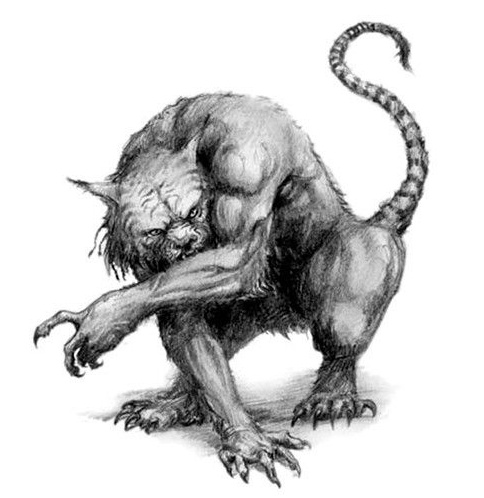
\includegraphics[width=100mm]{./fig/trollcat.jpg}

\vspace{2 cm}


\normalsize
completed campaign    \\
cleanup whenever

\vfill

\today

\end{center}






%-------------------------------------------------------------------------------
% copyright etc on the back side of the title page
%-------------------------------------------------
\clearpage
\thispagestyle{empty}
\raggedbottom

\vsmall
\noindent
This work is licensed under a Creative Commons \\
Attribution-NonCommercial-ShareAlike 4.0 \\
International License. (CC BY-NC-SA 4.0).\\
\url{https://creativecommons.org/licenses/by-nc-sa/4.0/} \\
\url{https://creativecommons.org/licenses/by-nc-sa/4.0/legalcode} \\
If you want to use it in any other fashion please contact the author.

\

\noindent
All images are temporary placeholders, \\
most are downloaded and unattributed.\\
They need to be replaced with licensed art.

\normalsize






%-------------------------------------------------------------------------------
% begin main matter
%------------------
\cleardoublepage
\pagestyle{fancy}
%\flushbottom
\raggedbottom



%--------|---------|---------|---------|---------|---------|---------|---------|
%       10        20        30        40        50        60        70        80
%-------------------------------------------------------------------------------
\section*{Eviction}
\markboth{eviction}{eviction}
%------------------
A stand alone adventure in three parts. Hunt down and get rid of Lord Majsan and her family. Things are not as they seem. It is easy to miss the quirk. A challenge for 4-6 Heroes around 250xp for a total party of 1000-1500xp.

\vspace{1.0\baselineskip}

\tableofcontents
\markboth{eviction}{eviction}

%\vspace{2.0\baselineskip}
%\vspace{3.0\baselineskip}
\vspace{5.0\baselineskip}

% ensure enough space left on page (XX lines), or flush a new
% \clearpage so as not to break the introduction too early
%\needspace{10\baselineskip}
% not needed if we put intro in minipage

%\noindent\begin{minipage}{\textwidth}
\phantomsection\addcontentsline{toc}{section}{Introduction}
\section*{Introduction}
\markboth{introduction}{introduction}
%------------------------------------
Lord Majsan and her people heard the rumours of strife and opportunity in the Pawa -- Conq region after the Troubles with that Green Demon. Finding the seat of a remote northern valley empty, they settled and are slowly rebuilding.

Upon discovery of the foreign force, Baron Conq sent an emissary to proclaim His Rule over the region. Majsan rudely refused. Now Baron Conq, via his elite military, is hiring The Heroes to sort out the issue of getting rid of the squatters.
%\end{minipage}

\vspace{1.0\baselineskip}


%-------------------------------------------------------------------------------
%\begin{samepage}
\noindent\begin{minipage}{\textwidth}
\noindent A notice on the job board in Trade Town reads:

%\

\begin{readoutloud}
Heroes Wanted! 200 silver for a week's work.

Baron Conq requests the aid of Capable\textsuperscript{*} Adventurers in evicting a gang of squatters from an old ruined keep up in the Kort Mountains. Their leader has refused to kneel and pay tribute and is therefore illegally occupying land which by King's Decree falls under the Domain of Baron Conq.

Meet Captain Lundqvist in Sleepy Cove for more information and your Bond of Employment.

\

\noindent
\textsuperscript{*} \small recommend a total strength of at least 1000xp \normalsize
\end{readoutloud}
\end{minipage}
%\end{samepage}
%-------------------------------------------------------------------------------

\vspace{2.0\baselineskip}


\noindent
This is intended as a small stand alone adventure, but can easily be inserted into a campaign. It adds the Tellgun lands and the village of Kort to the region, but has no other significant influence. Regardless of how it turns out.


\subsection*{synopsis}
%---------------------
The Heroes take the contract, get some provisions, and travel into the mountains on the way to Tellgun's Keep. At the Old Toll Watch they don't pay and take a fight. Beata Blodig and Majsan flee and carry word to both the Mine and the Keep, possibly bringing a few wounded Ruffians.

Following the NW road the Heroes reach the Keep, which is now on alert. They can try sneaking up at night to silently scale the walls. Fight the warband, but it is likely that at least Malvina will escape to the Mine. Hopefully they manage to kill Fake Majsan.

Mission successful they travel back and get paid. All done. Until a few weeks later when they are tracked down and told to finish the job. Majsan is still alive! WTF?

The Heroes go back, the Keep is again manned. They ask around in the valley and village of Kort. Find out about the Mine and go there to fight Black Haired Majsan. The real one. Majsan and Malvina may escape to come back and make trouble in future adventures. The Heroes do not get paid extra for their additional work.


\subsection*{sisponys}
%---------------------
This adventure can take some odd turns and twists. The path above is just a likely example. Their guide, Kvitten, can point them in a direction, discuss and argue, but should not be forceful. And Kvitten does not know about the Mine or Fake Majsan. She can just barely navigate the region and will not help them fight.

Never rely on your players to do what \textit{you} think is likely and obvious. They will catch you with your pants down. I've added extras and options. Who knows, they might even decide to join Majsan and ditch Kvitten. That way they might survive until Lundqvist has the time to root out the Keep.


\subsection*{background}
%-----------------------
Lord Majsan is leading the band now that their mother Malvina has taken to Trolling and is no longer as reliable a leader as she used to be.

Majsan brought a couple of scouts with her and travelled the area incognito to understand the situation. Talking with the farmers of Tellgun's lands and the people in nearby Kort it becomes evident that Baron Conq has never had any interest in the area and that Power and Law was always Lord Tellgun. Until Those Demon Problems, where Lord Tellgun and most of his men were slaughtered by some otherworldly monster just passing through.

Since the death of Tellgun the area has gone down hill fast. The last few men of the household guard are staying in the keep, not venturing out cleaning the land from dangers. The people are living in fear and many have died from various horrors encroaching upon the land.

This can be an important aspect of this adventure. The people of the mountains, the Kort villagers, the farmers of Tellgun's lands, and those who used to work Tellgun's mine are very happy that Malvina's daughters have arrived. The newcomers have gone hunting monsters and also brought some silver with them. They are also working to get the mine going again, bringing work and income. They have even started patrolling the roads to keep them safe. The people have never in practice lived under rule of Baron Conq, even if Lord Tellgun's lands are clearly in Conq's domain.

The Conq barons has never bothered with the Tellgun lands. They have very little value and are mostly just dangerous. The reason Baron Conq even bothers is because of the insult of some self proclaimed Lord settling and refusing to subjugate herself.


\subsection*{future}
%-------------------
For the time span of this adventure, Baron Conq and his military are occupied with the recent Bandit Problems, see \texttt{Goblin Destiny}. They have no time to apply force against the newcomer up in the uninteresting nowhere. Hence hiring Heroes.

This will not last. If the Heroes fail and the problem persists, Baron Conq will eventually task Lundqvist with getting rid of Lord Majsan. That will be the end of the story. Such military action will, if necessary, take place after the adventure concludes, after Lundqvist has successfully gotten rid of the Goblin Bandits.


\subsection*{region}
%-------------------
The North Kort Mountains, Lord Tellgun's Lands, etc, all poor and lost, overrun by monsters and misfortune. Eisenkrafs lost a lot of wealth when Gebbhard Goebbels died during \texttt{Return of Uchly Namen} and no new leader has gotten the mine running properly yet. Lord Tellgun was no master of wealth and economy, but kept the region somewhat safe, until he got eaten. Since then it's gone downhill fast.

The locals, miners and farmers, are generally very happy that a strong warband has taken up the banner and go out making the roads safe again and trying to open the old Tellgun Mine. The ones who have met Red Haired Majsan are commonly impressed by her charisma and power. Only four old miners have met Dark Haired Majsan, and they only think she is the new Mining Boss. All locals think Red Haired Majsan is the Leader of the Warband, and their new Lord.

Local people, especially those working for Lord Majsan, often say she treats them well, that she is the Best Boss Ever. They tell stories about earning wages, having food, hope, safer roads, possible work with the mine, etc. They are honest and open about their support. Regular hard working people who see the hope of better years ahead.


\subsection*{the new lord}
%-------------------------
Majsan is sly, brutal, unscrupulous. The region is already lousy with monsters and crap, but to make it worse she has also hired some orcs and goblins to terrorise Tellgun's Valley and Kort Village. They steal cattle and children to eat, and burn a couple of farms. Majsan won't let them make too much of a mess. Red Haired Majsan will ride out and get rid of them in a showy manner after some time. All this to guarantee the support of the local population. These Svartfolk are from the foreign east and do not speak much Common. It is however possible to find foreign silver coins from the Eastern Lands in their coffers, indicating that there is something strange afoot. If they are captured and interrogated in Svartlingo they will say the thin dark woman has paid them to eat children and burn farms.

Contrasting the local people, the original ruffians and the hired bandits are coarser and more nasty. Majsan has told them to keep quiet and stay back but they will still throw derogatory remarks and crude jokes at the Heroes. They will laugh at their misfortunes or "obvious stupidity". They will shout and threaten but will take a moment or two of restraint before firing off physical aggression, unless provoked.


\subsection*{both of them}
%-------------------------
To successfully complete the adventure the Heroes need to get rid of both the Fake and Real Majsan. If they kill just one, the other will come back after the Heroes leave and continue to fortify and settle.

Likely ways to get rid of them is to either show enough force that Majsan consider the region not worth the effort, or to kill both. Enough force is to kill both Malvina and Gosan and most of their henchmen. Lesser losses can be recouped by recruiting from the Valley or village of Kort, where Majsan has a strong reputation and the poor and hardy population likes the new Lord.

Kvitten will think that it is all over if the Heroes manage to drive off Fake Majsan, since as far as she knows Red Haired Majsan is the real Lord Majsan. That's enough to get paid. But a couple of weeks later Lundqvist's people will hunt them down and say the problem is not solved and that Lord Majsan is still alive. Lundqvist will force them to fix the issue. A few nights in Conq's dungeon cells might persuade reluctant Heroes.


\subsection*{derailroad}
%-----------------------
When I write adventures I often add plenty of options and alternative solutions for the players so they feel, and are, in control of their experience. That doesn't mean the world is adapted for their level of potency. Some optional side quests will be easy, others lethally dangerous or even impossible on first attempt. I signal by having the world around react to the dangers in various ways. Gossip, travel difficulties, attempts of sealing up access, corpses of previous brave souls, etc. In the end it should be the players' decision, and I prefer to present more options than the narrow railroad needs.

Two extra adventures, the SW Darkness at the Old Toll Watch and the Mine Tunnels at Tellgun's Mine are available but too dangerous to complete immediately. They are intended for more experienced Heroes to return to at a later date, as side quests in some other adventure, etc.
Included here as bad options. The danger is signalled by the fact that the villain bosses have spent significant resources to close off both areas. Hint strongly about danger if the Heroes pursue, but let them stumble to their death if they are careless. Carefully investigating is not inherently lethal, just very dangerous. The SW Darkness is easier to escape. The Mine Tunnels is more insidious and actively trap exploring Heroes.

A handful of wilderness fight encounters are are also included in case the Heroes work for Lord Majsan somehow and need to go hunt monsters. The mountain wilderness is dangerous and full of critters. If the Heroes spend time out there they will encounter animals, monsters, demons, goblins, etc.

Encounters not used can be recycled later on.


\subsection*{choice}
%-------------------
The Heroes might just decide that they are hired by the wrong side in the conflict, flip and work for Majsan instead. Let them. But when looked at closely, Majsan's gang is brutal and horrible. The Heroes might well flip back again and say it was all an elaborate ruse.

Working for Lord Majsan they will see Red Haired Majsan leading her Warband, probably meet Malvina, troll strange, and probably at least see Gosan talking with Majsan. The Real Black Haired Majsan will never be seen outside the Mine, she presents as just the Mine Boss.

Lord Majsan has use of fighters. She will send them on more and more dangerous cleaning tasks. Monsters out in the wilderness, then the demons in the SW Darkness and the Mine Tunnels. She is unlikely to send support with them.
%But Gosan might be interested to come with for the Mine Tunnels and the South West Darkness, though she will make sure to stay behind in relative safety most of the time.
%NOTE Gosan probably should not go with the Heroes without proper escort, the Heroes are new and not fully trusted with the core family.
There are multiple encounters available here, and just make more if it suits you.

If the Heroes actually survive all that it is probably time for Lundqvist to attack with a huge military force after a bit of peace and quiet. Majsan's core people will die or flee, and the Heroes will never see them again. Lundqvist is likely to either execute turncoat Heroes, or put them to forced labour. Effectively ending the mini campaign. Suggest not playing out the Lundqvist assault. Simply describe the force closing on the Keep. Perhaps the Heroes are quick and stealthy enough to escape...







%--------|---------|---------|---------|---------|---------|---------|---------|
%       10        20        30        40        50        60        70        80
%-------------------------------------------------------------------------------
\phantomsection\addcontentsline{toc}{section}{Meeting in Sleepy Cove}
\section*{Meeting in Sleepy Cove}
\markboth{sleepy cove}{sleepy cove}
%--------------------------------
The Heroes find passage to Sleepy Cove for 10c per head and 20c per horse, wagon, or other large items. The ship sails with next morning tide and ties up at Sleepy Cove dock in the evening. A fast and windy passage, have Heroes roll con or suffer mild sea sickness mod-1 until after a night's sleep on land.

Sleepy cove is a quaint little village where life is slow and relaxed. The Heroes will notice that a most of the people look a whole lot like each other. Love your family and all that. The villagers seem happy. They wave and say hi unless the Heroes look exceptionally blood thirsty or ready to attack. Sleepy Cove is described in more detail in \texttt{Return of Uchly Namen}.

Anyone in the village knows that Captain Lundqvist and a few of his soldiers are waiting at the village inn, Sleep with the Fishes, since the day before.

\

Entering Sleep with the Fishes immediately presents Captain Lundqvist at a table talking with a hired spellslinger. His powerful retinue seated at the next table. He looks up when the Heroes enter and asks if they have come for the Eviction Job? If so he bids their leader to sit with him and quickly explains the situation.

\begin{readoutloud}

[Captain Lundqvist]: Some foreign Warlord, Majsan, is squatting in a northern valley. She has taken over Tellgun's Keep after the old fart managed to get himself eaten a while back. The stupid man must have been peckerweak because he left no heirs. Not even a single unknown bastard claiming the seat.

Anyhow, we are busy with a lot of bandits at the moment, so we'll pay you 200 silver to go up there and get rid of the foreigners. She has refused to subjugate and pay tribute to Baron Conq, so you can kill her or kick her out, whichever is easiest.

I'll send Kvitten with you (pointing at a light infantry soldier). Her life is worth more than all of yours combined. She will not be taking any heavy fights for you.
You will get paid when she is satisfied.

All Clear? Off you go!

\end{readoutloud}

He continues talking with the spellslinger about hunting down the bandit gangs festering in the SouthWoods and surrounding region. Captain Lundqvist hangs around for an hour or so then leaves.

\

Kvitten presents herself. Seems nice but stern. No nonsense. She will help guide them for any necessary shopping the next day, recommending that the Heroes stay here at the inn for the night.

She can describe Tellgun's Keep as a small stone fortification on a bluff overlooking a small valley with some farmland. It sits along the mountain road, a few leagues from the village of Kort. Tellgun used to have fewer than 10 strongmen to keep the road and region safe, so there can't be too many people in the Keep.

Lord Majsan has rudely rebuffed the requests of the Envoy Baron Conq sent to notify her that she was settling under his Dominion. Kvitten doesn't know more about the self appointed Lord than what the Envoy has told the military. A strong red haired woman with a rude brutish behaviour.

\

\noindent
Gossip in Sleepy Cove, success:
\begin{description}
    \item[-3:] There are demons everywhere! Stay Safe!
    \item[-3:] Some foreign traders caused a fight in Kegern. Trying to sell stolen goods, they say.
    \item[0:] There are bandits in the SouthWoods. Goblins! Lots of them! We need more patrols to keep the roads safe. Farmer Beard lost two sacks of grain a while back.
    \item[0:] There is a lot of trouble around these days. Captain Lundqvist is here to recruit a specialist spellslinger to root out the goblins in SouthWood. And Innkeep Smallbeard said they have also sent for more people to go up in the Kort Mountains.
    \item[+3:] Trader Jakob says the whole Burmak Guard marched out on the Kegern Moors to hunt bandits. And never returned! Dark Days!
    \item[+4:] Aah, you must be here to take care of the ruckus up at old Tellgun's Keep? I heard some foreign Lord settled there with their warband. Malvina's Daughters I think they said. Malvina is some big bandit out East.
\end{description}

Followup on the gossip story of Malvina's daughters: Some trader told the tavern about a large bandit Eastward, Malvina, who had two daughters.Her gang was driven off recently and the trader was happy. The tavern keep later heard about large women settling in Tellgun's Keep, and assumes it must be Malvina's daughters.

\

% The histography roll is modified because this is a foreign gang.
\noindent
Histography mod-3, success:
\begin{description}
   \item[0:] Malvina was an old bandit leader. Successful and with a nasty temper. She used to run a gang of some 20 bandits for a long time and effectively carved out a piece of land to rule.
   \item[1:] They were active out East for decades, but has not been heard of for a while.
   \item[3:] She had two daughters: Majsan, the oldest, capable and clever, and Gosan, more of a big brute.
   \item[4:] Malvina's Daughters never go anywhere without their big murder cats.
\end{description}

\

When the Heroes enter Sleep with the Fishes the first time they might notice the rough goblin sitting drinking by herself: \\
At the bar, silently, sits a goblin. Keeping to herself but presents as Guthrud Grönskinn if pressed. Tries to stay out of trouble. This is Hemskelina, the terrifying scout of GamGang, see \texttt{Goblin Destiny}. All incognito. She has infiltrated several villages in the region as itinerant help and scout. She helps merchants and caravans travel safely and avoid the scourge of the bandit gangs. This way she can lure targets into the most lucrative raids, but mainly she hears a lot of juicy information.

If asked she says she can't help people up north. She only knows the SouthWoods and roads around Sleepy Cove, Merna, Kleinshof.








%--------|---------|---------|---------|---------|---------|---------|---------|
%       10        20        30        40        50        60        70        80
%-------------------------------------------------------------------------------
\phantomsection\addcontentsline{toc}{section}{Old Toll Watch}
\section*{Old Toll Watch}
\markboth{toll watch}{toll watch}
%------------------------
A relatively light encounter. Pay or fight. Beata will ride to notify the Keep and Mine of a fight or noteworthy Heroes, unless caught.


\subsection*{synopsis}
%---------------------
The Heroes will either pay 3c per head and pass peacefully, or choose to fight. Either way messages will be sent to both the Keep and the Mine that a band of Adventuring Heroes are in the region.


\subsection*{background}
%-----------------------
Once, ages long lost, it was a temple and tomb of some divine ruler or some such. No one knows. Histography-6 will inform of "God Emperor Lucipants, who ruled by divine right and wrought shadow spears from the souls of his subjects", but that's not true.

The old tomb behind the temple has been looted and empty since forever. Tellgun started using it as a small fort to house his patrolmen when they were keeping the roads clean of monsters and murderers.

The SW tunnels lead to a dungeon tomb, infested with monsters. Gosan lost a ruffian to some horror, then sealed up the entrance. Majsan placed a warning beacon which triggers if something comes out, or if someone tries to remove the blockage.

\

Majsan's people has been cleaning up the roads from bandits and monsters, and Red Haired Majsan has hired two old miners to work as toll masters. They are very thankful for the work and happy with the new Lord. They have never met the real Majsan.

\

The road forks at the Old Toll Fort. If asked, Kvitten will argue that the troublesome squatter is holed up in the keep following the NW road. They should go there first to evict her. No sightseeing. They are on the clock and under contract. But she will neither debate nor force the issue. She doesn't know that the NE road leads to Tellgun's mine, or that the real Lord Majsan is holed up there to get the mine up and running again. She has never been in this uncivilised outland, and only been told what the returning envoy said: Lord Majsan is holed up in Tellgun's Keep and refuses to subjugate herself.


\subsection*{talking with the toll master}
%-----------------------------------------
If the Heroes pay their toll the Toll Master is very happy to chat with them a bit. He is open and friendly and talks well of Lord Majsan, the cleaning of the roads, future safety and prosperity for the region, etc.

The ruffians from Majsan's original Warband are more obnoxious and will laugh or insult the Heroes given the opportunity. But they have orders to stay back and behave. They won't get physical unless provoked, and Gosan will step out to keep them in line if they go overboard.


\subsection*{map mechanics}
%--------------------------
The Heroes can either pay 3c per head and be on their way peacefully, or fight. The Ruffians and Gosan will try to enforce payment. If a fight goes against them they will flee. Beata Blodig rides to notify Majsan in the Mine, Gosan flees to the Keep. The Ruffians scatter and regroup at the Keep.

Notifying the Mine fast is top priority. Beata Blodig will ride fast, or if she has fallen Gosan will go instead, or send one of her panthers. Notifying the Keep is secondary and will be done by Gosan, a Ruffian, or one of the panthers.

Opening the heavy stone doors to the temple the Heroes are back-lit and cannot see into the darkness. The heavy arbalest operator will be able to fire on stationary target (anyone busy opening the door) for a round or two. There are two doors, it takes 30/str rounds (ru) to open a door enough to a normal guy to slip through, 25/str for small, and 20/str for tiny. For plate armour and bulkier it takes 40/str. Two guys can squeeze together to help with each door. While they are pushing they are considered as stationary targets for the arbalest shooter. So the arbalest shooter is firing at mod+3 (aimed, short, stationary) and have two loaded arbalests at ready.
The other doors in the temple are 20,15,10/str, 30/str for bulky.


\subsection*{opposition}
%-----------------------
The Toll Master and Night Watchman are old miners from Eisenkrafs. They will try to not engage unless they are sure they can win, fight only in supporting fashion, and they will try to flee if things turn sour. The Night Watchman will fire both ballistas if cornered in the temple then try to hide and escape.

The Ruffians, loyal henchmen, will fight if they think they can win, and escape around half hp. They know that they have to bring word to both the Keep and the Mine. They can escape into the mountains and are very tricky to find in that terrain.

Beata Blodig will give support fire with her bow, then ride off to bring word to the Mine. This signals that the Keep is not the most important place. Or, it can get people thinking that there are other hidden roads in the mountains that allow travel between places. Also true.

Gosan and her panthers will fight ferociously but escape around 33-50\% hp. She has run away reserve and some of her mothers fast healing from Troll Blood.


\subsection*{loot}
%-----------------
This is an outpost. The only valuables are basic equipment, provisions, and weaponry. Most opponents will flee and not leave corpses to loot.
The two heavy arbalests in the inner temple are very valuable if the Heroes can bring them.
The rest is kit for the toll watch staff, about a week's worth of simple living.









%--------|---------|---------|---------|---------|---------|---------|---------|
%       10        20        30        40        50        60        70        80
%-------------------------------------------------------------------------------
\phantomsection\addcontentsline{toc}{subsection}{The South-West Darkness}
\section*{The South-West darkness}
%---------------------------------
Available as a bad-idea option for the players. They should take the hint of danger. If they push forward recklessly they will probably be wiped out. Give them plenty of hints: thoroughly blocked, magic protection, dark, smells of death, uneasy feeling (roll psy), etc. Avoid and come back later, in another campaign.


\subsection*{synopsis}
%---------------------
Hopefully they will escape soon after encountering a wraith, rather than wake them all, or annoy the vacationing demons.


\subsection*{adventure}
%----------------------
The Heroes can investigate the sealed off darkness dungeon, which is way too dangerous for them and will probably lead to a party wipe if they are not careful. Gosan have sealed off the crypt for a reason. It is too dangerous.

Three Demons bathing in the polluted pools. They have entered through the rift pool in the innermost room, and are mostly just hanging out and relaxing. Some annoying weakling came in a while back so they played with it then killed it. Wasn't good eating. The restless spirits create a fun ambience.

A wraith wakes and emerges from a sarcophagus if trespassers delay too long nearby (3sq 5r), if the crypt is disturbed or defiled, or if another wraith gets hurt. Effectively fighting any wraith will wake all of them. They will coordinate and focus on anyone who has managed to hurt one of them, or defiled their resting place.


\subsection*{map mechanics}
%--------------------------
The rift pool in the innermost room is a side effect of the summoning of Uchly Namen, see \texttt{Return of Uchly Namen}. Dive through to other weird adventures elsewhere, or perhaps just an unknown death. Not covered here.

Any relevant disturbance of the tomb will wake at least one Wraith. Hurting any Wraith will wake all of them. Living presence close to a sarcophagus (3sq 5r) will wake that Wraith.

The Demons are relaxed and don't want to be disturbed. They don't like the humans or other weaklings, not good eating, annoying vermin, just kill it. Play with it for a bit if it makes fun noises.

The SW Darkness magical alarm device: It will signal Gosan and Majsan when disturbed. It activates either when something passes by out from the sealed off crypt, or if someone stays in the 3sq detection range for more than 3r.
Turning off the device is a magic roll.


\subsection*{opposition}
%-----------------------
The Wraiths will be dangerous to anyone with low psy if they don't have magic weapons or armour.

\noindent Wraiths\\
These ghostly undead can not be hurt by non magical weapons nor blocked by non magical shields and armour. They can also pass through walls and attack from within walls. They slowly seek straight line to their target and makes one attack per round. They use scream to try to scare away people that manage to hurt them, or groups of attackers even if they don't hurt them.

Even a bit of magic helps. E.g: casting stafflight on a weapon or shield will give a little bit of damage chance. Perhaps a mana 1 stafflight gives 30\% damage chance with half damage done.
Even if barely magical stuff do not damage a wraith they will recoil and move away from the hit.


\noindent Demons\\
The vacationing tourists are here for relaxation and blood sport. They don't like intruders that make their hotel scream, but will be happy to play with them until they fall apart.


\subsection*{loot}
%-----------------
The crypt has some statues, small and large, that have value to collectors. They can be found here and there as decorations in niches along the walls. The sarcophagi have valuables buried with their owners. Battle gear, jewellery, trinkets.

The items are old, but to collectors in Trade Town they might be worth 5+1d20 gold per sarcophagus. In the local villages the price is perhaps a quarter of that. The weapons and armour are unusual custom items. All need repair or suffer mod-3, but they are of excellent quality.










%--------|---------|---------|---------|---------|---------|---------|---------|
%       10        20        30        40        50        60        70        80
%-------------------------------------------------------------------------------
\phantomsection\addcontentsline{toc}{section}{Tellgun's Keep}
\section*{Tellgun's Keep}
\markboth{the keep}{the keep}
%------------------------
An assault or sneak infiltration? How to get into a small but defended keep?


\subsection*{synopsis}
%---------------------
The Heroes come to the keep to evict Majsan. Fight, sneak, or otherwise to get in. Search for Majsan. Fake Majsan either escapes or is killed. Malvina probably escapes. Perhaps Gosan has fled here from the fight at the toll fort, if so she will probably escape as well.


\subsection*{adventure}
%----------------------
Talking with the farmers in the valley they find out that the population in the region are happy with the new Lord and her protection and investments in the Keep and the Mine. Gossip-3 can find someone who has a gripe with the Lord but no one who has enough ire to do anything against her. Same in the village of Kort.

Instead the population want the Heroes to focus on helping Lord Majsan to clean out the Mine so a few of the men can start working there again. Coin is short.


\subsection*{infiltrate}
%-----------------------
If the Heroes don't attack, perhaps they will try to infiltrate to gather information? Presenting friendly or asking about work they will be well greeted and let in, provided they leave their weapons at the door. Lord Majsan will be charming and friendly. She talks openly about the misfortune of the land and how she is rebuilding. She will not mention the Mine. She says they are fighting monsters everywhere and she will happily pay per monster head they can bring her. For small monsters she will pay 3c, medium sized are worth 5c and larger worth 10c per head.

Present Lord Majsan as a skilled and charismatic leader, busy with building a future. She scoffs at Baron Conq: \textit{Do you see any Conq soldiers here? No? Why are they not patrolling the roads or keep the villagers safe?} No, she is here to rule and rebuild. She will not bow and pay tithe to some absentee lord.

If the Heroes accept her terms for work she will set up tents for them inside the castle, until they have built new housing. She will immediately send them out to hunt down monsters in the area. \textit{Just go out and kill monsters. There are lots of them.}


\subsection*{map practicalities}
%-------------------------------
The scale of the map is odd. At the burnt in grid the main barn is only from ca 7x3m to ca 35/15ft depending on sq size approximations to 1.0m / 1.5m / 5ft. Either way it's small. Setting double grid size gives a better size, and all ramparts and stairs are two man wide.
Either or. 1x grid gives a tight cramped fight and 2x grid gives quite a lot of space.


\subsection*{map mechanics}
%--------------------------
It's a small old keep. The walls are not high and in poor repair. 4r climb-3. during the climb anyone on the wall is mod+3 to hit from above with spear or similar.

Crenellations give full cover when the defenders hide behind them. They give mod-6 protection when shooting out from behind them, and mod-3 protection when people are running around on the parapet.

The main house is two floors, access through ladder, with the top floor just filled tightly with beds.

A 100sq escape tunnel lead from the stone larder to a hidden spot in the NW rocky terrain. The entry point in the larder is hidden under a crufted shut stone trapdoor and no one knows about it any more except the mad groundskeeper and the old housekeeper.

During the night there are normally two guards walking the parapet on and off. If the Keep is on alert there are also two ruffians or Guzman's gang awake and ready. Malvina may be outside the Keep stalking the land.


\subsection*{sneaking in}
%------------------------
Scaling the walls in cover of darkness can be a good idea. Fewer guards and ruffians are out and about, and once the alarm is sounded it takes a while for people to emerge and get battle ready.

Declaring and successfully rolling dungeoneering and track, both at mod-6, can theorise and locate a hidden 100sq escape tunnel which comes out in the floor of the stone larder, potentially right beside a sleeping Majsan. Majsan will wake up when they hack open the crufted shut stone trap door.

Bribing an angry farmer to help smuggle them in under a wagon load of hay will cost 100s or so. But first they need to find an angry farmer since most are happy with the new Lord.


\subsection*{loot}
%-----------------
Thoroughly searching the keep there is old battle gear for 10 soldiers (mod-1 until repaired). Lord Tellgun's old plate armour, shield, and sword. The cash box of Fake Majsan is hidden away under the floor in the kitchen corner (find-3), containing 5g 90s 150c. Besides the family, only the housekeeper knows about it, and she is truly honest and highly loyal to the new Lord.

200enc of assorted tools, materials, gear worth 500c. Food for 200 portions, etc.








%--------|---------|---------|---------|---------|---------|---------|---------|
%       10        20        30        40        50        60        70        80
%-------------------------------------------------------------------------------
\phantomsection\addcontentsline{toc}{section}{Tellgun's Mine}
\section*{Tellgun's Mine}
\markboth{the mine}{the mine}
%------------------------
Tellgun's Mine map is mostly for variation. Some interesting choices to be made by the players regarding access, scouting, strategy.


\subsection*{synopsis}
%---------------------
Gain entry, scout, fight. The ringleaders will try to escape if pressed. Malvina will fight to the death to protect her daughters. The family will team up and be smart. Their cats are very effective in the low light.


\subsection*{adventure}
%----------------------
Probably the final battle with the Malvina's Daughters. If the Heroes just walk up they will be noticed and everyone will be on alert, ready to fight. Majsan will have at least one clever idea in place on how to fight the by now well known Hero Party. The mine does not have any back entrances and is easy to defend. If possible Majsan will have moved the mounted heavy arbalests from Old Toll Watch to the mine. If given time she might also have hired a couple of sell swords or some orc or goblin fighters.


\subsection*{background}
%-----------------------
Majsan, some ruffians, and some old miners are starting to get the mine back up and running again. They know there are dangerous demons in the old mine tunnels so they have torn down the rail bridge. Majsan will use the proceeds from the already existing ore to hire people to go clean out the lower mine shaft and get rid of the PinkLarge rumoured to be living there. \textit{She doesn't know there are more than one}.


\subsection*{map mechanics}
%--------------------------
The elevated small passages are crawl spaces. Small Heroes (goblins, halflings) can crawl through at speed/3, normal sized (human, elf, dwarf) at speed/6, large (orc or human str or con $\geq9$) or armoured (abs $\geq$2) cannot get through. Requires a climb action to get up to crawl spaces.

Majsan has recently moved into the mine to try to get it up and running again


\subsection*{opposition}
%-----------------------
Majsan, some ruffians on watch, and some old miners inside, plus anyone who has fled here from the Old Toll Watch and Tellgun's Keep. Hence, the opposition strength depends largely on how many people managed to escape the earlier fights.

They have likely gotten word about the Heroes and also knows the composition and strength of the party. Majsan is clever and will turn any information about the intruders to her advantage when she plans the defence.


\subsection*{loot}
%-----------------
The Family's treasure chest is hidden away in a false shaft covered with dirt, find-6. It contains 15g 200s 200c. With it is also hidden two of the magical alarm devices. Only Majsan and Gosan knows how to operate them.

There is about 100enc of materials and tools, worth 200c. Some 5000enc in ore worth 1c/enc. About 50 rations worth of provisions.









%--------|---------|---------|---------|---------|---------|---------|---------|
%       10        20        30        40        50        60        70        80
%-------------------------------------------------------------------------------
\phantomsection\addcontentsline{toc}{subsection}{Mine Tunnels}
\section*{Mine Tunnels}
%----------------------
A bad option possibility for the Heroes. They should take the hint and not go down here. Give them plenty of red flags: baaad feeling, smells like death, the bridge was deliberately razed, etc.

Preferably this is a place the Heroes come back to at some other time when they are stronger, or just insert it in a future adventure.


\subsection*{synopsis}
%---------------------
If they are not careful to secure escape routes they will die here. The demons are hungry, numerous, sap stamina, and and can move fast in their hidden tunnels.


\subsection*{adventure}
%----------------------
A PinkLarge demon have settled in here and started breeding. By now they are 3 adults and lots of small pinklings. They are happy to get snacks walking into their maze-like den and will let the intruders in quite a bit before surrounding for an ambush. They will fight to the death to defend their lair. They have no way to escape unless the Heroes actively funnel them out through the entrance tunnel.


\subsection*{map mechanics}
%--------------------------
This is a "bad" battle map, but gives a weird cramped feeling since there is no light and lots of narrow winding tunnels. Here and there are about 20 "deep pit into darkness", which are entry point to strange biological slimy pink tunnels. The demons can move very fast between the entrance points and the Heroes can't follow. Trying to crawl into a tunnel is ooze vapour poison effect str9 draining dam2 stam3 each round. Elves are immune to poisons, but the tunnels will contract and fight back str10 for each sq the hero tries to move.

Upon entering they notice the noxious stench. Pass con roll or take whole fight at max stamina -1. Roll monsterology for the smell. Success:\\
=0: smells like demons, more than one.\\
+3: PinkLarge lair, they are toxic, and breed pinklings.\\
+4: Known to lure people in and surround them.\\
+5: Penetrating claw attacks.\\
+6: Can travel through organic tunnel networks.\\
+7: If left alone they will grow into PinkHuge monstrosities.

Most of the floor is broken stone, poor terrain mod-3.
Trying to move on the broken ground is always a dex+9 balance roll (mod-3 => dex+6+balance) on first movement each round. Allow for a "recover balance action" if the heroes fail the first roll each round, costing 3ap and 1/3(ru) of their remaining mp.
Or they can move carefully, paying double mp for every sq of movement. But allow for 1sq movement, safely, each round.

Roll per-3 each 10r to find evidence of small slimy pink growths in the dark crevices. Active: find+3. Close to the deep pits into darkness the slime is more common, per-0, find+6. Same on the south part of the map.

Roll per-6 each 10r or track+3 / find+3 shows that there are spiky "footprints" of light things walking on hard large claws. In the SE \& SW areas it's +6 instead of +3 and there are now also heavy footprints from huge claws.

Peeking into a deep pit into darkness without holding ones breath gives oozing vapour poisoning str5 vs con doing dam0 draining stam1.


\subsection*{opposition}
%-----------------------
All the demons sap stamina which makes it even more difficult to run away. The monsters can almost always run faster and get behind the Heroes, cutting off the retreat. Most fighting will probably be melee base contact where also the pinklings ooze vapour and sap stamina.

The PinkLarge will mostly stay in the SE \& SW region, but can pop up to block an escape on the north part if necessary. They don't want their food to escape.


\subsection*{loot}
%-----------------
There is no relevant loot here except the bodies of the demons. They will be worth 2g each for the right buyer. But they have to be wrapped tightly in oilskin and carried on stretcher or wagon far behind a horse and downwind. The poison vapour will kill over time.








%--------|---------|---------|---------|---------|---------|---------|---------|
%       10        20        30        40        50        60        70        80
%-------------------------------------------------------------------------------
\phantomsection\addcontentsline{toc}{section}{Wilderness}
\section*{The Wilderness}
\markboth{wilderness}{wilderness}
%--------------------------------
Travelling the wilderness for fun or profit is hazardous. Apart from the normal monsters and wild things living or roaming the region, Lord Majsan has paid goblin raiders go around attacking farms as well as an orc bandit gang to go after travellers and merchants on the roads.







%--------|---------|---------|---------|---------|---------|---------|---------|
%       10        20        30        40        50        60        70        80
%-------------------------------------------------------------------------------
\phantomsection\addcontentsline{toc}{subsection}{Goblin Raiders}
\section*{The Goblin Camp}
\markboth{goblins}{goblins}
%--------------------------
These raiders are here to cause havoc. Live well on livestock and children, burn some farms, loot some stuff. Then they expect to leave with some well earned silver in their pocket, having been paid for a job well done.


\subsection*{adventure}
%----------------------
If the Heroes go out scouting for monsters to kill they can pick up the trail of the raiders, leading away from a burnt down farm. The farmers crying over their two kidnapped children and ask the Heroes to help save them.
With a clear trail (track+3), the Heroes follow the raiders to their camp. Kill, slaughter, loot. The children are dead and one is partially eaten.


\subsection*{information}
%------------------------
These goblins are foreigners. They were hired back east and travelled here for a light one season job. They don't speak much Common, but knows an Eastern dialect of Svartlingo, mod-3 against the normal.

If they manage to capture a raider and forcefully question him in Svartlingo (mod-3) he will eventually say that the thin dark woman hired them to come here to eat children and burn farms.

Real Lord Majsan has hired them to raid the outskirts of Tellgun Valley and Kort Village. Majsan plans to have Fake Majsan slaughter them all to cement the support of the local population. She will poison a festive offering and provide plenty of strong wine. A few hours later Red Haired Majsan and her Warband will ride in and slaughter them all, followed by wide eyed hired farmers and miners.


\subsection*{loot}
%-----------------
The raiders don't have much. Some basic supplies, all equipment is worn, most stuff is of too poor quality or repair to fetch a useful price. But, hidden in the spider box is their small treasure chest, with 15s 240c, as well as a small bag of 30 silver which look very strange. Foreign Eastern Silver, paid by Majsan as an advance for their work. They have been promised another 100 silver after the season is done.

Note that it would be theoretically possible that the Eastern Silver actually come from a raided farm or merchant, or from earlier. Red Haired Majsan will just shrug and feign ignorance about it if asked.


\subsection*{reporting}
%----------------------
Coming back to Lord Majsan and reporting of slaughtering the goblin raiders she will for a brief moment let her mask slip and flash anger. Let the Heroes roll per-3 to notice it. She will thank and pay them as usual though. If questioned about the slip she will just deny it.










%--------|---------|---------|---------|---------|---------|---------|---------|
%       10        20        30        40        50        60        70        80
%-------------------------------------------------------------------------------
\phantomsection\addcontentsline{toc}{subsection}{Orc Bandits}
\section*{Orc Bandits}
\markboth{orcs}{orcs}
%---------------------


\subsection*{adventure}
%----------------------


\subsection*{information}
%------------------------


\subsection*{loot}
%-----------------


\subsection*{reporting}
%----------------------










%--------|---------|---------|---------|---------|---------|---------|---------|
%       10        20        30        40        50        60        70        80
%-------------------------------------------------------------------------------
\phantomsection\addcontentsline{toc}{subsection}{ScreamHisser Demon}
\section*{The ScreamHisser Demon}
\markboth{demon}{demon}
%--------------------------------
This tourist is here on vacation, enjoying the scenery and exotic cuisine. The Summoning of Uchly Namen made it easy for other travellers to enter for a while.
For the players it is hopefully an interesting and different fight, it has no intended relevance to the story. Included here in case the Heroes go out hunting monsters.


\subsection*{opposition}
%-----------------------
The ScreamHisser randomly spawns small shadow vines every now and then in his vicinity. The area already has them scattered about before the fight starts.

The Demon won't immediately attack. He has no languages in common with the Heroes but is interested in them until they start to pose a threat by surrounding him, attacking, or similar.

When attacked he will react with a shimmer shield which will perhaps turn the hit to a miss. Next turn he will start summoning horned chargers then a stone form or two. If given time he will stick around, laugh, play, summon lots of shadow vines, perhaps fight a bit for himself. He doesn't pursue fleeing Heroes, and can happily start pulling a fallen Hero apart while the others slowly walk away.

If dropped to low hp he will fly away and escape.

\

Shadow Vines are attracted to strong psyche and will prefer to attack high psy Heroes before others, and will prefer to move towards them if close by. If caught by the snares the vines will eventually overwhelm the target and drain mana and psy until the victim is comatose. The victim will never wake up by itself if captured by vines and feinted.

\

Horned Chargers weigh more than several men and have the height of a large boar. Highly aggressive. They try to charge and impale on the horns then later pin down to gore and bite the wounded victims. A horn charge fail by -1 or -2 is a knockback 1 hit instead dam3.

The horned chargers will heal from death in about an hour, and even grow a new body from the head after a few hours. They will break bags or become too heavy to carry after a bit. If kept they will attack again as soon as they have grown new legs. If cut into pieces only one piece will grow a new horned charger. The other pieces will simply rot away to noxious slime in a few hours.

\

Stone Form is simply puppeteered animated rocks. No intelligence or instinct. Will perform as instructed by the master. The ScreamHisser has a mental link which costs him 1ap per stone form each round to maintain. He will not keep more than four active at any time since that will force him to overdeclare +2ap and still be able to summon other stuff.


\subsection*{loot}
%-----------------
When killed the vines just evaporates and the stone form are just rocks. But the horned chargers heads can be collected, as can the head of the ScreamHisser.


\subsection*{later}
%------------------
If the Heroes come back to the site the ScreamHisser will probably have returned. He likes the place. This time he will either fight them for real, or fly away immediately, depending on how it turned out last time. He will always flee instead of stay and risk death.

If he get angry enough he may spy on the Heroes and set a trap, attack when they are wounded or beset by other monsters. Then giggle and fly away when the main offender has been killed.









%--------|---------|---------|---------|---------|---------|---------|---------|
%       10        20        30        40        50        60        70        80
%-------------------------------------------------------------------------------
\phantomsection\addcontentsline{toc}{subsection}{Wolf pack}
\section*{The Wolf Man and his pack}
\markboth{wolves}{wolves}
%-----------------------------------
A Wolf Man Warrior out hunting with his wolf pack has caught the scent of the Heroes. He will have his wolves chase the Heroes to him in an open glen, where he intends to fight them in open battle and make trophies of them.

The encounter has nothing to do with the rest of the story, and is here to provide a different kind of fight to entertain the players if they have their Heroes travel around in the wilderness.


\subsection*{opposition}
%-----------------------



\subsection*{loot}
%-----------------
If the Heroes are out hunting for Lord Majsan they can collect for the heads, and she will pay double for the wolf man warrior, since he has been menacing the local population for quite a while.







%--------|---------|---------|---------|---------|---------|---------|---------|
%       10        20        30        40        50        60        70        80
%-------------------------------------------------------------------------------
\phantomsection\addcontentsline{toc}{subsection}{Mutts and Bats}
\section*{Mutts and Bats}
\markboth{harried}{harried}
%--------------------------
Returning or fleeing from another fight, wounded, tired, they are sniffed out by a pack of carrion mutts and soon the hunt is on. The Heroes are run down in random light woodland terrain and both the carrion mutts and a murder of carrion bats chase them through a 50-60sq gauntlet.
It is meant that the Heroes should try to escape since some of them are wounded. Balance based on how fast they can pass and how many can fight.


\subsection*{map mechanics}
%--------------------------
Make the Heroes roll for track+3, or int-3, to figure out that it is important to get through the map in a specific direction. Escaping the map randomly will put them in elevated danger of the faster monsters continuing to hunt them down. They need to escape to the safe exit region.

Escaping elsewhere and they will just be hunted down soon again with their max stamina reduced, and by even more hunting carrion animals. The Heroes are wounded and smell like easy food for all the hungry teeth and maws around.


\subsection*{opposition}
%-----------------------
Carrion Mutts and the larger Carrion Hounds will run around attacking with claws and bites, but try not to stay in melee. The bats fly by fast and do claw attacks then fly on, as a fast swarm. When they find a severely weakened target they will cling and bite.

\

Carrion Mutts and Carrion Hounds:\\
The smaller Carrion Mutts will run down the Heroes, claw and snap at them, but make sure to always have 2ap left to escape from melee immediately after the target's right to react action.
The larger Hounds will take melee fights with weaker targets. Try to bite and clamp giving mod-3 and continuous auto thrash hits.
\small \begin{verbatim}
claw   11 2ap dam6
bite    9 4ap dam8 pen4 + option to clamp down hold: gives target mod-3
thrash  auto hit damage 6 pen 4, keep clamped
\end{verbatim} \normalsize

\

Carrion Bats:\\
The bats come in groups, streaming past in quick fly-by attacks. When the victim seems to be getting weaker they start landing and cling on to overwhelm and drink it dry.
\small \begin{verbatim}
fly-by claw attack: W12-0 R15-1 D18-4     claw 8 mod-abs  dam1 pen99
   make sure the bat has at least a few mp left after the
   attack, to fly out of range of the target immediately after
   it has taken the right to react action.
fly-avoid 5
land-cling  9    no damage   target mod-2 per clinging bat
cling-bite  7 mod-abs   1dam/r pen99
   once a cling bite attack is successful the bat continues drinking
   automatically 1dam/r for max 5r, then it is full and flies away.
   The cling mods to target persists while the bat sucks away.
\end{verbatim} \normalsize

%\

\subsection*{loot}
%-----------------
If they are working for Majsan they can take some heads if they stop long enough to cut them off. The bats are so tiny that Lord Majsan will only pay 1c/head.











%--------|---------|---------|---------|---------|---------|---------|---------|
%       10        20        30        40        50        60        70        80
%-------------------------------------------------------------------------------
\clearpage
\phantomsection\addcontentsline{toc}{section}{appendix: allies}
\section*{The Good Guys}
\markboth{allies}{allies}
%------------------------
Kvitten is the only relevant allied npc, and she is not intended to bloody her spear. She will not take part of any fighting if she has a choice. Let her stay and watch the horses or wait by the escape route.

Kvitten is a very powerful light infantry soldier. The whole Lundqvist force is presented in \texttt{Goblin Destiny}. Lundqvist's unit is elite military, the tip of the Conq spear, an insurmountable do-not-fuck-with force which normal Heroes cannot reasonably challenge. \textit{But of course they have tried.}
\textit{If I ever write a Super Heroic $>$1000xp campaign arc opposing Baron Conq I'll probably use Lundqvist force as a boss fight.}




%-------------------------------------------------------------------------------
\begin{samepage}
\phantomsection\addcontentsline{toc}{subsection}{Kvitten}
\subsection*{Lundqvist Light Spearman -- Kvitten}
%------------------------------------------------
Kvitten is very fast with strong defence and a serious bite. She is not tasked with fighting for real on this milk run, just help guide the Hired Heroes and observe.

\

\small \begin{verbatim}
========== Lundqvist Light, human ==========
str  8                    hp 20 abs 2
dex 10                    m2 w5 r8 d12
con  8                    stamina 12
int  7                    vision 25 day 240
psy  8                    mana 6
per  8                    action points 7
cha  6                    xp ?
--------------------------------------------
synchronised 8, combat group lundqvist & lundqvist-light
spear 12, slash, fancy 4, wayward strike, counter attack, charge 6
throw 9, brawl 5, intercept, opportunity, consistent 1, precise 1
shield 12, fast defence, phalanx guard
avoid 9, yield+3, dodge+3, off balance
mobile 5, rapid 6, veteran 4, balance 6, tank (chain as leather)
quickdraw 8, quaff 8
Common 8
--------------------------------------------
money: 15 silver, 20 copper
quaff 4x in quickdraw
heavy spear, lundqvist fine, mainly 1h + shield,  1h/2h
    dam 7/8, pen 0/1, abs 12, parry-1/+1, reach 1 mod-2
    str 7/6 (str bonus max +2 dam then max +4 pen)
    slash: mod-2, dam-1
    finesse-4/-6
large shield, lundqvist fine
    abs 20, parry+4,
    str 7, or slow 1 str 4
    Ranged attacks mod-3 when in the way.
    Hiding behind it (3ap) ranged mod-6
    tackle mod+2
chain mail  abs 2 (tank : chain as leather)
\end{verbatim} \normalsize
\end{samepage}

%\














%--------|---------|---------|---------|---------|---------|---------|---------|
%       10        20        30        40        50        60        70        80
%-------------------------------------------------------------------------------
\clearpage
\phantomsection\addcontentsline{toc}{section}{appendix: opposition}
\section*{appendix: Opposition}
\markboth{opposition}{opposition}
%--------------------------------
We have the main head honchos in Majsan, her sister Gosan, and their mother Malvina. They run their warband of ruffians, now bolstered by local bandits, miners, farmers, and the Guuzmar trio. Assisted by the wizard Hoher, more like an uncle than a hireling.

The Monsters out in the mountains or in the crypts and caves; vacationing demons, goblin raiders, hungry animals, etc all plague the area. Some belong to the story, but most are just available for player choice side missions.




%-------------------------------------------------------------------------------
\phantomsection\addcontentsline{toc}{subsection}{The Family}
\subsection*{Majsan, Gosan, Malvina, Fake, Beata, Hoher}
\markboth{family}{family}
%-------------------------------------------------------
Malvina's family all have a little bit of Troll blood. They heal fast between fights and they all have the battering ability. They are also surviving bandit leaders and have learned to put emphasis on getting out of trouble, so they all have run away reserve.


\goodbreak
%\clearpage
\begin{samepage}
%\phantomsection\addcontentsline{toc}{subsection}{Malvina}
\subsection*{Malvina}
%--------------------
Malvina will attack with little care until low on hp, at which point she escapes by run away reserve and recovers in a few days. She has some troll blood in her and heals 10hp/day. She also goes a bit crazy every now and then, and now in her later years she is going more troll all the time.

\

%\begin{samepage}
\small \begin{verbatim}
Malvina -
================== human ===================
str 11(8)                 hp 26(19) abs 0
dex  6(4)                 m1 w3 r6 d8
con 11(6)                 stamina 11(9)
int  7                    vision 16 dusk 180
psy  8                    mana 9
per  7                    action points 6(3)
cha  4                    xp 3 (610)
--------------------------------------------
troll blood: con+5, heal 10hp/d, dusk vision, smell-y-vision 5sq
--------------------------------------------
quick 3, mobile 2, rapid 3                                 45+12+13
strong 3, agile 2, resilient 7, enduring 2                 18+8+49+4
balance 3, veteran 5                                       9+25
Common 8(3), gossip 7, haggle 9, count 4, literate 3       27+24+40+8+4
avoid 8, yield +3, off balance                             64
axe 11, double 6, accurate 1, charge 3                     108+36+10+9
leader 7                                                   49
run away reserve, battering, black cat 2, luck 2           15+30+4+4
--------------------------------------------
2x axe + double 6
great axe  11 3(4)ap  dam 12, abs 14, parry-4, toparry-3, toavoid+2, finesse-2
1h            3ap  str 6 slow 1, str 9 dex 6 normal speed
           10 4(5)ap  swing: slow 1 mod-1 dam+4 toavoid+2
money: 1 gold, 11 silver, 8 copper
\end{verbatim} \normalsize
\end{samepage}

\





\clearpage
\begin{samepage}
%\phantomsection\addcontentsline{toc}{subsection}{Lord Majsan}
\subsection*{Majsan}
%-------------------
Leader of the gang since a few years now that Malvina is unreliably Trolling too often. She found the pretty and spectacular Elvira Slaktare at a theatre and hired her to be the face of the gang, playing the role of Lord Majsan - The Barbarian Queen!
Everyone from the old eastern gang knows the truth, but it is very effective when dealing with outsiders. And it gives Majsan a safety buffer.

\

%\begin{samepage}
\small \begin{verbatim}
Majsan -
================== human ===================
str  7(6)                 hp 20(17) abs 2
dex  6(3)                 m1 w3(2) r6(5) d12(9)
con  6                    stamina 11(8)
int  8                    vision 17 day 192
psy  7                    mana 8
per  7                    action points 6(3)
cha  9                    xp 101
--------------------------------------------
strong 1, agile 3, resilient 3, enduring 3, fast 3
quick 3, mobile 2
Common 8(3), gossip 7, haggle 9, count 4, literate 3
spear 10,
avoid 7, yield +3, off balance
battering, black cat 2, luck 2
--------------------------------------------
money: 2 gold, 1 silver, 8 copper

large spear 2h      high quality -50% abs str+1, sharp dam-1 pen+1
large spear         dam 6/6, pen 1/2, abs 12, parry-1/+1, reach 1 mod-3
1h/2h               str 6/5 (str bonus max +1 dam then max +3 pen)
                    slash: mod-2, dam-1 (long blade slash mod-1 dam6 pen0)
                    finesse-4/-6
brigandine abs 2
\end{verbatim} \normalsize
\end{samepage}


\begin{samepage}
\subsection*{shadow lion}
%------------------------
Intelligent and mind linked with Majsan. The lion will move through shadow to stalk vulnerable targets, or help Majsan when useful. Knockdown to gain advantage then bite.

\

%\begin{samepage}
\small \begin{verbatim}
knockdown so target have mod-3 and lion has mod+1 to attacks
weighs 300kg

knockback 2 str10
knockback 1 str15
tackle str20
knockdown str15

can move through darkness at 20sq/r
darkness is anywhere the heroes can't see due to lack of light
\end{verbatim} \normalsize
\end{samepage}








\clearpage
\begin{samepage}
%\phantomsection\addcontentsline{toc}{subsection}{Gosan}
\subsection*{Gosan}
%------------------
Very large and strong, she stands a head above most and twice as wide. With a huge custom hammer and two strange panthers she can take on a small group without much issue. She has some of her mother's fast recuperation and naturally heals 6hp/day.

\

%\begin{samepage}
\small \begin{verbatim}
Gosan -
================== human ===================
str  12(9)                hp 24(19) abs 0
dex  7(4)                 m2 w4 r7 d10
con  6                    stamina 13(9)
int  5                    vision 20 day 200
psy  9                    mana 4
per  5                    action points 5(4)
cha  6                    xp 101
--------------------------------------------
quick 1, mobile 2,
strong 3, agile 3, resilient 5, enduring 4, rapid 3
balance 2, veteran 4,
Common 8(3), gossip 7, haggle 9, count 4, literate 3
hammer 11, tackle 4, charge 3, consistent 1
avoid 8, yield +3, off balance
battering, black cat 2, luck 2
--------------------------------------------
money: 2 gold, 1 silver, 8 copper

huge 2h hammer 11   10 3ap: dam 9, toavoid=0, finesse-4
custom str10        11 4ap: dam 12, toparry-1, toavoid+1, finesse-3, knockback 1
abs 22, parry-3     10 5ap: dam 15, toparry-2, toavoid+2, finesse-2, knockback 2
2x5xp specialisations: tap (3ap), knock (5ap)
\end{verbatim} \normalsize
\end{samepage}


\begin{samepage}
\subsection*{panthers}
%---------------------
They are intelligent and mind linked with Gosan.
These panthers have incredible active fur camouflage. It's a per-3 roll each round to keep track of them even when in clear line of sight, =0 if also within perception range.
Opponents can spend a 3ap action to get +3 to the per roll to nail down where one is when in line of sight. Detecting by sound or smell is per-9 inside perception range, out of sight, and impossible further away.

Attacks when they are not successfully "tracked" are treated as surprise attacks, even if they are clearly within sight of the target, and the target does not get right to react.
They are automatically noticed if they are within sight and in base contact, but not in time to remove surprise if they move in to attack from outside base contact.

They are mobile and will team up on an opponent, often knocking down or distracting the target so Gosan can smash it with the hammer.

\

%\begin{samepage}
\small \begin{verbatim}
ap9: 1 attack 2 avoid
m3 w6 r10 d15, mobile 4, can run even if severely damaged
avoid 8 yield+3
claw  10 dam 2
bite   7 dam 5
knockdown 7 str 6 +1/sq charged, max str 12, dam 2, charge 6
\end{verbatim} \normalsize
\end{samepage}








\clearpage
\begin{samepage}
%\phantomsection\addcontentsline{toc}{subsection}{Fake Majsan}
\subsection*{Fake Majsan}
%------------------------
Fake Majsan enjoys playing the role of Warlord, and will step up if Real Majsan is dead. Malvina and Gosan will let her continue as the outwards Face, but Gosan will rule from behind.

Fake Majsan is very convincing as the Barbarian Queen Warlord and her interactions with the warband flow just like if she was the actual leader. Real Majsan, Gosan, Malvina take care of serious discipline, planning, etc, but Fake Majsan is getting better at it and can improvise well. She is smart enough to know when she definitely needs to call for new orders, and when she can take important decisions herself.

\

%\begin{samepage}
\small \begin{verbatim}
Fake Majsan - (Elvira Slaktare)
================== human ===================
str  9(6)                 hp 17(14) abs 2
dex  8(5)                 m2 w4(3) r6(5) d12(9)
con  5                    stamina 10(7)
int  8                    vision 17 day 192
psy  6                    mana 3
per  8                    action points 6(3)
cha 11(9)                 xp 10 (560)
--------------------------------------------
strong 3, agile 3, charming 2                            18+18+8
resilient 3, enduring 3, fast 3, rapid 2, charge 3       9+9+18+6+4
quick 3, mobile 2                                        45+12
balance 3, veteran 3, jump 4, acrobatics 4(8)            9+9+8+64
axe 10, double 5, fancy 3, consistent 1                  90+25+9+15
avoid 12, yield +4, off balance                          115
Common 8(6), gossip 3, haggle 3, count 2, literate 2     14+4+4+2+2
act 8  - theatrics -                                     32
luck 1                                                   1
--------------------------------------------
battle axe   10 3ap  dam 8, abs 10, parry-2, toparry-2, finesse-4, str 5
1h            9 4ap  swing: slow 1 mod-1 dam+2 toavoid+2
              8 3ap  poke: mod-2 dam-3 pen+2
great axe    10 3(4)ap  dam 12, abs 14, parry-4, toparry-3, toavoid+2, finesse-2
1h              3ap     str 6 slow 1, str 9 dex 6 normal speed
              9 4(5)ap  swing: slow 1 mod-1 dam+4 toavoid+2
partial plate abs 2 avg custom
money: 2 gold, 1 silver, 8 copper
\end{verbatim} \normalsize
\end{samepage}






\clearpage
\begin{samepage}
%\phantomsection\addcontentsline{toc}{subsection}{Beata Blodig}
\subsection*{Beata Blodig}
%-------------------------
Part of the family, sort of adopted. She's the messenger and a good regional scout. Blood thirsty and has developed the affectation of making sure she gets plenty of her enemies blood splashed or smeared all over her, and won't wash it away for at least a day.

Spending most of the time on horseback, she keeps her distance and pelts opponents with arrows until they are downed enough to go in for the kill using spear as a light lance.

\

%\begin{samepage}
\small \begin{verbatim}
Beata Blodig
================= human 2 ==================
str  5                    hp 13 abs 1
dex  11(9)                m2 w4 r6 d11
con  5                    stamina 9
int  6                    vision 19 day 266
psy  4                    mana 2
per 10                    action points 3
cha  8                    xp 113
--------------------------------------------
mobile 3, agile 2, rapid 3, veteran 2, balance 3, charge 4
ride 9, jump 4, mounting jump
bow 9, quick shot 3
spear 7, quickdraw 5
avoid 7, yield +4, off balance
Common 6,
--------------------------------------------
bow  (1r:9,3r:10) dam 4, pen 1, range 14, str 4
spear  7 dam 5/5, pen 0/1, abs 6, parry-1/+1, reach 1 mod-3  (2h parry 8)
1h/2h    str 4/3 (str bonus max +1 dam then max +2 pen)
         (pen3 riding as lance) x3 quickdraw from horse
leather armour  abs 1
money: 3 gold, 4 silver, 15 copper
\end{verbatim} \normalsize
\end{samepage}



\clearpage
\begin{samepage}
%\phantomsection\addcontentsline{toc}{subsection}{Hoher}
\subsection*{Hoher}
%-------------------------
Strange wizard who have been part of the family for many years.
He uses his offensive levitate to hoist opponents off the ground so they can't run away or close to attack, while others shoot them full of arrows or something. If things really go wrong he can teleport away to his basement in a cabin far away by crushing his escape token, in 1r. He won't be back for at least 10 days after that, if ever.

\

%\begin{samepage}
\small \begin{verbatim}
Hoher - the robed one
================= human 2 ==================
str  5                    hp 13 abs 0
dex  6                    m1 w3 r6 d9
con  4                    stamina 7
int  8                    vision 19 day 266
psy 10                    mana 16
per  4                    action points 4(3)
cha  4                    xp 4 (260)
--------------------------------------------
quick 1, mobile 2, rapid 2, veteran 1                         5+12+6+1        24
ride 4, jump 2                                                8+4             12
spear 8, accurate 1                                           57+10           57
avoid 5, yield +3, off balance                                20              20
Common 6, literate 6, counting 4, histography 6               18+18+8+18      62
spellcaster, magic 3, power casting 2                         20+18+4         42
black cat 1, luck 1                                           1+1              2
--------------------------------------------
teleport  8  2r 1m line of sight                              21              21
levitate  7  1r 1m range 10+5/m duration 3r+2/m, speed 3sq    16              16
             each round: psy-vs-psy or land, dex to not fall
--------------------------------------------
quaff 1x
high quality spear, +50% abs, requires str+1
spear    8  dam 5/5, pen 0/1, abs 9, parry-1/+1, reach 1 mod-3
1h/2h       str 5/4 (str bonus max +1 dam then max +2 pen)
            slash: mod-2, dam-1
            finesse-4/-6
crush-item  teleport home  1r
money: 2g 12s 25c
\end{verbatim} \normalsize
\end{samepage}









%--------|---------|---------|---------|---------|---------|---------|---------|
%       10        20        30        40        50        60        70        80
%-------------------------------------------------------------------------------
\clearpage
\phantomsection\addcontentsline{toc}{subsection}{The Warband}
\section*{The Warband}
\markboth{warband}{warband}
%--------------------------
The charismatic Majsan and Fake-Majsan have gathered loyal henchmen and hangarounds through their travels and from Tellgun valley. The bravery and loyalty varies quite a bit between the groups. Most will flee early rather than fight to the bitter end.

%\


\begin{samepage}
\subsection*{Ruffians}
%---------------------
Ruffians are experienced loyal henchmen Malvina and her daughters have accumulated through the years. They will fight to low hp before they try to flee. A few might even fight to the death, especially to protect Fake-Majsan, who has won serious affection of most of the gang.

\

Based on standard hireling, switch to axe and regular shield, bow, leather,
more mobile, less skilful no phalanx,
add bow secondary, extra luck , add black cat
\small \begin{verbatim}
===================================
str 5         hp 15 abs 1
dex 7         m1 w3 r6 d8(9)
int 4         vision (human average)
psy 4         mana 2
per 6         ap 5(3)
-----------------------------------
quick 2, mobile 2, resilient 2, enduring 1, veteran 2, balance 1
axe 8, shield 6, avoid 8, yield+3, off balance, swing
bow 6, ballista 3
luck 2, black cat 1
-----------------------------------
1h axe 8
   dam 7, abs 8, parry-3, toparry-1, toavoid+1, finesse-3
   str 4 (max +4 str bonus)
   swing: slow 1 mod-1 dam+2 toavoid+2
shield 9(6)
   abs 10, parry+3, tackle+1, str 4
   Ranged attacks mod-2 when in the way. Hiding behind it (3ap) ranged mod-4
bow 6  (1r:3 2r:6 3r:7)
   dam 4, pen 1, range 14, str 4 (no str bonus)
leather armour abs 1
   str 1 (str penalties affect all actions)
   dash-1, acrobatics mod-1, martial arts mod-1, sneak mod-1
   spellcasting mod-1, swim mod-1
money: 1d3s 10+1d10c
\end{verbatim} \normalsize
\end{samepage}

%\


\begin{samepage}
\subsection*{Bandits}
%--------------------
Ex Eisenkrafs Bandits. These guys have scraped by since their band was murdered off in \texttt{Return of Uchly Namen} and have now joined Lord Majsan. They keep a low profile for a while until they get a good feel for their new group.

They will fight well but run away when wounded or seriously threatened. Opportunistic, they will abandon Majsan if it seems her Lordship will fail.

\

\noindent
Based on RoUN eisenkrafs bandits, levelled-up a little
\small \begin{verbatim}
===================================
Eisenkrafs bandit archer    (token)
-----------------------------------
str  5    hp 12 abs 1
dex  6    m1 w4 r7 d12
int  4    vision (human average)
psy  5    mana 3
per  7    ap 4(3) (1r bow, 2x dagger, 6ap-2: 3x dagger or 2x avoid)
----------
quick 1, mobile 2, sneak 7
dagger 5, avoid 8 yield+3
bow 8, quick shot 3, quickdraw 2 (bow,dagger)
----------
bow 8 (1r-0, 3r+1), 20 arrows in quiver
    dam 4, penetrating 1, str 5 (no str bonus)
    range 14, short 7 mod+1, long 24 mod-3, vlong 30 mod-6 dam-1,
              extreme 35 mod-9 dam-2,
dagger 5
    dam 3, abs 4, parry-1, toparry-2, toavoid-1, finesse-9
    str 2 (no str bonus), fast+1 if str 3 and dex 5
    first two attacks don't require stamina
    poke: mod-1 dam-1 pen+1
money: 5+1d10c
\end{verbatim} \normalsize
\end{samepage}

%\


\begin{samepage}
\subsection*{Old Miners}
%-----------------------
Old Miners have come from the old Tellgun mine and from Eisenkrafs. They are generally out of work and don't see any possibility of prosperity elsewhere. They will fight to perhaps 50\% hp before they try to slink away. They won't engage until after the leaders have started fighting.

\

\small \begin{verbatim}
===================================
str 4         hp 9 abs 0
dex 4         m1 w3 r5 d7
int 4         vision (human poor)
psy 6         mana 2
per 4         ap 4(3)
-----------------------------------
quick 1, mobile 1, veteran 2, balance 1
axe 12, avoid 8, yield+2, off balance, accurate 1
some have ballista 6
-----------------------------------
1h hack-axe 11(12)       mining tool: double damage to rock, metal, wood, etc
   dam 4, pen 2, abs 12, attack-1, parry-3, finesse-2
   str 4 (max dam+2 pen+2 str bonus)
   swing: slow 1 mod-1 dam+1 pen+1 toavoid+1
money	3+1d5c
\end{verbatim} \normalsize
\end{samepage}

%\


\goodbreak
\begin{samepage}
\subsection*{Farmers}
%--------------------
Farmers come to sell food and wares, and to earn some minor coin as day workers for the family. The keep needs a lot of fixing-up. They won't engage until after the leaders have started fighting, and there seems to be a reasonable chance to win. They will flee once below 66\% hp, they are not used to fighting.

\

\noindent
Take typical farmer stats from the book, equip with axe / spear / knife / bow.
\end{samepage}






%-------------------------------------------------------------------------------
\goodbreak
%\begin{samepage}
\phantomsection\addcontentsline{toc}{subsection}{Guuzmar gang}
\subsection*{Guuzmar gang}
\label{sec:guuzmarstats}
%-------------------------
The Guuzmar gang: Guuzmar, Okmok, Kek are hireling orcs that have sold themselves for cheap for a while when they don't have much else interesting to do. They are not loyal enough to fight to their last breath, and will flee if one of them fall towards half hp or if the situation turns seriously dangerous for either of them. They all have run away reserve and dash around 8-9.

All three will fight in a tight formation so Kek can defend the archers long enough for them to switch to melee weapons if necessary.

\

\noindent    % roll 6 select 3
Guuzmar : heavy bow and heavy melee\\
Okmok :  long bow and fast melee\\
Kek : very heavy melee and acts as deterrent
%\end{samepage}

\


%\clearpage
\goodbreak
\begin{samepage} \small \begin{verbatim}
Guuzmar  -
================== orc 1 ===================
str  8                    hp 19 abs 0
dex  3                    m1 w4 r5 d8
con 11                    stamina 13(11)
int  5                    vision 17 dusk 171
psy  7                    mana 7
per  3                    action points 4(3)
cha  2                    xp ?
--------------------------------------------
veteran bonus +1, brawl bonus +2
--------------------------------------------
Common 4, Svartlingo 6
quick 1, mobile 2, enduring 2, veteran 2(1+1)
sword 7, double 5, bow 8, quickshot 3, brawl 4(2+2), strength bonus
avoid 6, NO YIELD, off balance
run away reserve 1, luck 1
--------------------------------------------
brawl bite: 4 dam 3 slow-1, gives +1 extra pain, mod+3 if grappled
brawl fist: 4 dam 2 fast+1
brawl kick: 4 dam 4
large bow (1r 8, 2r 8, 3r 9) dam 5, pen 2, range 16, str 6 (no str bonus)
large sword 7 dam 8, abs 14, str 6 (max +3 str bonus), finesse-6
   poke: mod-1 dam-1 pen+1
   swing: slow 1 mod-1 dam+2 todefend+2
parry dagger 7 dam 3, abs 8, attack-1, parry+1, finesse-5
   str 2 (no str bonus), every second attack in a round costs no stamina
   fast 1 if str 3 and dex 5
   poke: mod-1 dam-1 pen+1
money: 12 silver, 25 copper
\end{verbatim} \normalsize \end{samepage}

\


%\clearpage
\goodbreak
\begin{samepage} \small \begin{verbatim}
Okmok  -
================== orc 3 ===================
str 13                    hp 18(14) abs 0
dex 10                    m2 w3 r7 d9
con  6                    stamina 14(12)
int  1                    vision 18 dusk 132
psy  1                    mana 8
per  7                    action points 4
cha  6                    xp ?
--------------------------------------------
brawl bonus +2
--------------------------------------------
Common 1, Svartlingo 5
mobile 2, resilient 4, enduring 2, veteran 2
sword 7, double 6, bow 8, quickshot 3
brawl 2(0+2), strength bonus
avoid 5, yield +1, off balance
run away reserve 1, luck 1
--------------------------------------------
brawl bite: 2 dam 1 slow-1, gives +1 extra pain, mod+3 if grappled
brawl fist: 2 dam 4 fast+1
brawl kick: 2 dam 6
large bow (1r 8, 2r 8, 3r 9) dam 5, pen 2, range 16, str 6 (no str bonus)
large rapier 7
   dam 5, abs 5, toparry-2, toavoid-1, finesse-9, str 4 (no str bonus)
   fast 1 if str 6 and dex 7, every second attack in a round costs no stamina
   poke: mod-1 dam-1 pen+1
parry dagger 7 dam 3, abs 8, attack-1, parry+1, finesse-5
   str 2 (no str bonus), every second attack in a round costs no stamina
   fast 1 if str 3 and dex 5
   poke: mod-1 dam-1 pen+1
money: 3 silver, 5 copper
\end{verbatim} \normalsize \end{samepage}

\


%\clearpage
\begin{samepage} \small \begin{verbatim}
Kek  -  Headharvester Kek
================== orc 4 ===================
str 10                    hp 18(15) abs 0
dex  7(6)                 m2 w4 r6(5) d8(6)
con  5(3)                 stamina 11(7)
int  5                    vision 17 dusk 143
psy  3                    mana 2
per  2                    action points 4(3)
cha  1                    xp ?
--------------------------------------------
veteran bonus +2, brawl bonus +3
--------------------------------------------
Common 2, Svartlingo 6
quick 1, mobile 2, resilient 4, enduring 2
agile 1, tough 2, fast 2, veteran 2(0+2)
axe 10, swing, avoid 10, yield +2, off balance
brawl 7(4+3), strength bonus
--------------------------------------------
brawl bite: 7 dam 3 slow-1, gives +1 extra pain, mod+3 if grappled
brawl fist: 7 dam 3 fast+1
brawl kick: 7 dam 5
large 2h axe  10
   dam 14, abs 13, parry-3, toparry-1, toavoid+1, finesse-3, str 8
   swing: slow 1 mod-1 dam+4 toavoid+2
money: 4 silver, 5 copper
\end{verbatim} \normalsize \end{samepage}

\








%-------------------------------------------------------------------------------
\goodbreak
\phantomsection\addcontentsline{toc}{subsection}{Goblin Raiders}
\subsection*{Goblin Raiders}
\label{sec:goblinstats}
\markboth{goblins}{goblins}
%---------------------------------------------------------------
The goblin raiders is a large gang with several trained wolves. Most are reckless and brave until they see at least a few comrades killed, at which time they will flee and regroup.

\

\begin{samepage} \small \begin{verbatim}
Goblins
\end{verbatim} \normalsize \end{samepage}

\

The wolves are standard from the book, two large and four regular. They will pack attack and drag down their target to bite and rend.
\begin{samepage} \small \begin{verbatim}
Wolves
\end{verbatim} \normalsize \end{samepage}

%\











%-------------------------------------------------------------------------------
\goodbreak
\phantomsection\addcontentsline{toc}{subsection}{Orc Raiders}
\subsection*{Orc Raiders}
\markboth{orcs}{orcs}
%------------------------------------------------------------
The orc raiders are a small experienced band Majsan has hired to run around the mountains killing and stealing for a season before returning east. They will be quick to flee if cornered or seriously wounded.

Throw in orc raiders as encounters along the roads, at bridges, crossings, etc, or as bolster to the goblins raiders. The two raider gangs are separate but know about each other and keep peace since they are both getting paid by Majsan for the same time. The orcs also carry a pouch with 30 silver in Eastern coin, just like the Goblin Raiders.

The orcs have a huge trained bear with them. The bear is fairly smart and very experienced fighter. He will figure out a reasonable action in most situations. For a bit part he functions as a scary focus for the opponents giving the orcs a chance to move in or away.

The orcs also have two donkeys with them that carries their tents, provisions, equipment, etc. The donkeys are usually tied up a bit away from their fights, off map, but can be tracked down mod-3. The donkeys are guarded by an old wounded orc who is also the cook / medic of the party.

The orcs speak svartlingo with an eastern dialect and know no Common.

\

\begin{samepage} \small \begin{verbatim}
===================================
orc raider
-----------------------------------
str 10    hp 20 abs 1
dex  6    m2 w4 r7(6) d9(8)
int  4    vision (orc average)
psy  4    mana 2
per  6    ap 5 (235)
----------
quick 2, mobile 2, balance 2, rapid 2, fast 2, veteran 3(1+2)
club 9, swing, brawl 5, str bonus, accurate 1, charge 3, tackle 2
shield 6, avoid 6, yield+3, luck 1, black cat 1
----------
large club  1h/2h   9
   dam 6/8, abs 14, parry-1, toavoid+1, finesse-2
   str 6 (max +3/+4 str bonus)
   1h: str vs str for knockback 1
   2h: str+3 vs str for knockback 1
   swing: slow 1 mod-1 dam+2 toavoid+2 knockback roll +3
shield     9(6)     tackle 3(2)
   abs 10, parry+3,
   str 4, or slow 1 str 1
   fast 1 if str 8 and dex 12 and fast shield 3
   Ranged attacks mod-2 when in the way.
   Hiding behind it (3ap) ranged mod-4
   tackle mod+1
leather armour abs 1
\end{verbatim} \normalsize \end{samepage}

\

\noindent
The bear is a larger stronger version of a large wild bear with some veteran and better attack skills.
\begin{samepage} \small \begin{verbatim}
===================================
large bear                  (token)
-----------------------------------
str 20    hp 40 abs 1 skin
dex  7    m3 w6 r10 d16
con 12    vision 15, sniff 20
psy 10    ap 4
per 14
----------
bite   12 (slow 4ap) dam 12 pen 2
claw   10 (fast 2ap) dam 8 knockback 1
avoid   4 yield+3
pain threshold 5, veteran 3
mobile 2, rapid 2,
charge  6, mobile 1, balance 6,
accurate 1
-----------------------------------
\end{verbatim} \normalsize \end{samepage}













%--------|---------|---------|---------|---------|---------|---------|---------|
%       10        20        30        40        50        60        70        80
%-------------------------------------------------------------------------------
\clearpage
\phantomsection\addcontentsline{toc}{section}{appendix: monsters}
\section*{Monsters in the Wild, the Crypts, and the Caves}
\markboth{monsters}{monsters}
%---------------------------------------------------------
The northern region is mainly a barren unpopulated mountainous expanse with a few small spots of inhabited land. Monsters and proponents of alternative life styles roam the region, commonly causing lethal problems for the few remnants of civilisation.











%-------------------------------------------------------------------------------
\goodbreak
\phantomsection\addcontentsline{toc}{subsection}{ScreamHisser et al.}
\subsection*{ScreamHisser, Shadow Vines, Horned Charger, Stone Form}
\label{sec:screamhisserstats}
\markboth{screamhisser}{screamhisser}
%-------------------------------------------------------------------
This is a simple combination encounter. The ScreamHisser demon likes the area and has stayed there for a while, unconsciously seeding it with Shadow Vines. He will summon Horned Chargers and Stone Form puppets as soon as the Heroes show any aggression against him. He has no

\

\textbf{The ScreamHisser} summons the other opponents. He is a tourist on vacation. More curious than blood thirsty. Do not play him optimally immediately when the fight starts. He will fly away when seriously wounded instead of fight hard.

\

\begin{samepage} \small \begin{verbatim}
ScreamHisser
6ap
claws 2ap  +deflect
scream 4ap
avoid 3ap
shimmer shield, bring up 4ap, lasts 3r
summon shadow vines 8 4ap
    immediately place success diff shadow vines, contiguous
summon cloud : horned charger  4ap  cloud duration 1r,
    then between rounds, when cloud disappear, make charger visible
summon cloud : stone form  4ap  cloud duration 2r
    then between rounds, when cloud disappear, make stone form visible
\end{verbatim} \normalsize \end{samepage}

\

\goodbreak
\textbf{Shadow vines} move slow but are many and difficult to spot. They start hidden om map and treat as sneak=0 when moving or sneak-3 when stationary: the Hero must succeed with a perception roll to spot vines creeping inside their perception range, or perception-3 to spot stationary vines inside their perception range.

Vines are mod=0 to attack with slashing weapons but mod-3 for piercing or crushing attacks. Vine attacks are parried at mod=0 with shields and mod-3 with other weapons.

\

\begin{samepage}
\small \begin{verbatim}
Shadow Vines
1 attack per round, reach 1,  snare or bite
move 1sq/r, cannot occupy smooth lit surfaces, dark/shadow/soil/vegetation
snare 6 str 5 per snare (cumulative: 5,10,15,...) only one snare per plant
    target mod-3 per snare when held, cannot move unless break free
    can snare one new target per round, can have many targets snared
    leech mana at end of round: (nr snares) vs psy to drain 1 mana
        drains 1 mana for all snares, not per snare
    snares cannot be parried, but can be blocked with tower shield or similar
    snares can be avoided as usual with no mods
bite 5 (+3 if snared)
    dam1 penetrating psy-1 "it took a bite of my soul"
    psy recuperates +1 per good night rest
takes no damage when hit by non-luminous weapons
    roll for light strength, success kills, e.g: candle 4, lamp 7, torch 10
    or 5hp damage on the ground/shadow the vine comes from also kills it
\end{verbatim} \normalsize
\end{samepage}

\

\goodbreak
\begin{samepage}
\small \begin{verbatim}
Horned Charger
charge at initiative+7 R-0 D-2
\end{verbatim} \normalsize
\end{samepage}

\

\goodbreak
\begin{samepage}
\small \begin{verbatim}
Stone Form
Each stone form costs 1ap each round to maintain by mind link.
\end{verbatim} \normalsize
\end{samepage}

%\





%-------------------------------------------------------------------------------
\goodbreak
\phantomsection\addcontentsline{toc}{subsection}{The Wolf Pack}
\subsection*{Wolf Man and his Pack}
\label{sec:wolfmanstats}
\markboth{wolves}{wolves}
%--------------------------------------------------------------

\todo cleanup

\

\begin{samepage}
\small \begin{verbatim}
--- the wolf man ---

hp 22
mobile 2
veteran 2
pain threshold 5
yield 4
consistent 1
precise 1

ap 6

M4 W6 R10 D16

claw 12 2ap dam4
bite 8 4ap dam7
avoid 8 3ap

"large, strong, agile, claws"

his acrobatics jump cost no mp

str 11          hp 22 abs 0
dex 14       m4 w6 r10 d16
con 8         ap 8
per 8 very good nose and ears

jump 4sq for free no roll, then 5sq:9 6sq:6 7sq:3    +soa/3  (speed of approach)
jump acrobatic claw attack    todefend-4
tackle 6   str 11  +soa/3
charge 3

veteran 2, pain threshold 5
avoid 8, yield 4, dodge 2

mobile 2

claw 2ap  11  dam4     +held if 6 vs str        bite+3 / claw held
bite 4ap    8  dam7 (held if 9 vs str, target mod-3, wresting free is dam3 penetrating per attempt)
tear 4ap   (after bitten, held, 4ap dam6 penetrating, no roll successs=0)

When wolf man makes an acrobatic claw attack he does not stop, and the target only has one action to react before the wolf man is probably out of reach again.
Attacking wolf man during an acrobatic jump is mod-4.
\end{verbatim} \normalsize
\end{samepage}

%\








%-------------------------------------------------------------------------------
\goodbreak
\phantomsection\addcontentsline{toc}{subsection}{Mutts and Bats}
\subsection*{Carrion Hounds and Bats}
\label{sec:carrionstats}
\markboth{carrion}{carrion}
%---------------------------------------------------------------

\todo cleanup

\

\begin{samepage}
\small \begin{verbatim}
--- bat ---
\end{verbatim} \normalsize
\end{samepage}

\

\goodbreak
\begin{samepage}
\small \begin{verbatim}
--- hound ---
\end{verbatim} \normalsize
\end{samepage}

%\










%-------------------------------------------------------------------------------
\goodbreak
\phantomsection\addcontentsline{toc}{subsection}{SW Darkness}
\subsection*{South West Darkness}
\label{sec:swdarkstats}
\markboth{wraiths \& demons}{wraiths \& demons}
%------------------------------------------------------------

\todo cleanup

\

\begin{samepage}
\small \begin{verbatim}
--- WRAITH ---
max hp 10
fixed init  8
blackknight 3
ap 3
M2 W4 R6 D8

touch-drain  att7 3ap
scream att8 3ap
avoid 0 3ap


"That ... that is ... not good !"


scary 5     psy+3 to advance, psy to attack melee, psy+3 to attack ranged

m2 + attack                              1 attack per round
r6 to get close when angered     charge in but no attack
jump back 3sq when damaged  -  dissolv and reappear quick 3sq back

attack: touch 7  10 vs psy, drain diff hp stam mana on success
                       cannot be parried or blocked by non magical
attack: scream 8   13-distance vs psy : fear until pass psy roll (mod+1/r): must flee
                           target has mod+3 if passed psy from previous attack

Once a wraith is damaged, or a tomb is damaged or defiled:
all wraiths will wake up, get angry, and attack the offender.

general : tohit-3 - whispy
normal melee weapons: damage diff attacker psy vs 10
normal ranged weapons : no damage
magic melee weapons : full damage + diff psy vs 10
magic ranged weapons : full damage

can move slowly (1sq/r) through walls and floor
\end{verbatim} \normalsize
\end{samepage}

\

\goodbreak
\begin{samepage}
\small \begin{verbatim}
--- DEMON ---

hp 25    abs 2
stam 15
dex 8
con 10
veteran 3
pain threshold 5
blackknight 1
yield 2
accurate 1
ap 6
M2 W4 R8 D12

claw att12 2ap dam4
punch att12 3ap dam5   knockback str15
feflect (takes half dam) skill-12 3ap
avoid 9 3ap

"big and burly with claws and teeth,
a bit scary"

scary 3
str 15  punch knockback 1
          grab-hold gives mod+3 to bite
bite is vampiric, heals dam/2 hp instant
\end{verbatim} \normalsize
\end{samepage}

%\








%-------------------------------------------------------------------------------
\goodbreak
\phantomsection\addcontentsline{toc}{subsection}{Mine Tunnels}
\subsection*{Mine Tunnels}
\label{sec:minetunnelstats}
\markboth{pink ones}{pink ones}
%---------------------------------------------------------------

\todo cleanup

\

toxic vapours - both tunnel air and pinklings, gassy corpses

pink tunnels, toxic, muscle motile, slippery,
burnable

\

\begin{samepage}
\small \begin{verbatim}
--- PINKLING ---

hp 8
dex 9
mobile 2
rapid 1
veteran 1
painthresh 3
yield 4
dodge 4
ap 6
M2 W4 R7 D11

claw att9 2ap dam4 pen2
bite att6 4ap dam6 pen0
deflect skill 9 2ap
avoid skill 10  3ap


"not large, but:
evil looking claws,
and frightening maw"

6ap-0 8ap-2 w4-1

oozing vapour: only in base contact, or in death cloud: each round in vapour:
   fighting in base contact: 3 vs con or take dam0 stam1
   death cloud: (0sq,1sq,2sq) 7/5/3 vs con or take dam 1 stam 2

takes half damage from piercing

claw 9  2ap dam4pen2
bite  6  4ap dam6   mod+3 / grab-hold
grab-hold str 7

can travel 15sq/r in pinktube tunnels between "deep pit into darkness" markers
\end{verbatim} \normalsize
\end{samepage}

\

\goodbreak
\begin{samepage}
\small \begin{verbatim}
--- PINKLARGE ---
set freesize ca 30% larger than sq

hp 40
dex 8
mobile 2
rapid 2
veteran 2
painthresh 5
yield 4
dodge 3
accurate 2
ap 6
M3 W5 R8 D11

claw att11 2ap dam6 pen3
bite att6 4ap dam8 pen0
deflect skill 11 2ap
avoid skill 6  3ap


"not large, but:
evil looking claws,
and frightening maw"

6ap-0 8ap-2 w4-1

oozing vapour: only in base contact, or in death cloud: each round in vapour:
   fighting in base contact: 3 vs con or take dam0 stam1
   death cloud: (0sq,1sq,2sq) 7/5/3 vs con or take dam 1 stam 2

takes half damage from piercing

claw 9  2ap dam4pen2
bite  6  4ap dam6   mod+3 / grab-hold
grab-hold str 7

can travel 15sq/r in pinktube tunnels between "deep pit into darkness" markers
\end{verbatim} \normalsize
\end{samepage}

%\

























%--------|---------|---------|---------|---------|---------|---------|---------|
%       10        20        30        40        50        60        70        80
%-------------------------------------------------------------------------------
\clearpage
\phantomsection\addcontentsline{toc}{section}{appendix: xp}
\section*{XP, Milestones, Achievements}
\markboth{xp}{xp}
%--------------------------------------

Here are suggested XP payouts for the adventure. I don't expect any playthrough to collect it all.
Payouts are based on balancing for around 4-6 Heroes. Divide the total XP by the number of Heroes, henchmen and other xp leeches.

Many milestones are specified as first solution and any forced later solution. By "forced later" we mean that the Heroes are forced, not by choice, to create another solution. E.g: paying the Toll Master the first time they pass the Old Toll Watch, then \emph{forced} to fight when passing at a later date.

All sections have a maximum total cumulative xp payout. Regardless of how many times and in what way and order the Heroes come back and sneak, talk, bribe, fight, or otherwise engage with that story section the total maximum xp given to them should not exceed this total cumulative maximum. E.g: First time they encounter the ScreamHisser they drive him off, gaining 20xp. Next time they kill him, but only get 10xp, since 20 of the total max 30 is already paid from the first fight.

This total maximum should also include session xp paid out. If they are five heroes spending two sessions to complete the section, gaining 4xp each per session, they have already gained 40xp for the section. So if it took them two sessions to kill ScreamHisser they have already been paid 10xp more than the total maximum, so they get no further xp reward.


\subsection*{session xp}
I suggest 3-5xp per session to each Hero. That way there is always some progression even if nothing is achieved. Deduct the paid session XP from the total payout of whatever goals they are working towards.


\subsection*{milestones}
Instead of xp per critter killed or specific outcome of discussions and items looted we assign xp to functional outcomes of events, like gaining passage, getting information, removing threats, etc.

Running through the straight forward typical path from the synopsis is around 350-400xp total, around 60-100xp per Hero.

\begin{description}

% 30xp
\item[Getting paid:] Getting paid for the mission is 30xp bonus, regardless if they have solved the real problem or not.

% 30xp
\item[Fake Majsan:] Figuring out that there is a Fake Majsan and a Real Majsan is worth 30xp.

% 50xp
\item[Actually completing the eviction mission:] Finally killing off or driving away Real Majsan, Gosan, and the Warband is worth 50xp bonus. This completes the main adventure. Don't hand out this experience unless you as GM actually close the eviction mission and decide that the Leaders and Warband will not return.\\
Saving some mop up of side missions like the SW Darkness, Mine Tunnels, or various monsters for later is ok.

% 50xp
\item[Old Toll Watch:] Any way to pass the Toll for the first time is worth 20xp total, even just paying and passing. Any forced later solution should be 10xp total.
%E.g: first time they pay to pass and get 20xp, next time they are forced to return and fight and get 10.\\
Somehow extracting useful information from the Toll staff is worth another 10xp total. E.g: by striking up a conversation, filthy bribery, or capture and interrogation.\\
Total maximum cumulative xp for cleaning out Old Toll Watch is 50xp. This excludes the SW Darkness.

% 100xp
\item[Tellgun's Keep:] Gaining entry to Tellgun's Keep is worth 30xp the first time, then 20xp if forced to find other ways later on.\\
Gathering significant information from the people at the Keep is 10xp total.\\
Driving out Lord Majsan and her warband from Tellgun's Keep is 50xp total.\\
Total maximum cumulative xp for cleaning out Tellgun's keep is 100xp.

% 70xp
\item[Tellgun's Mine]
Finding out that the Mine exists is worth 10xp.\\
Finding out about Real Majsan is rewarded above, not from the Mine xp.\\
Total maximum cumulative experience for cleaning out the Mine, excluding the Mine Tunnels, is 70xp.

% 40xp
\item[SW Darkness] Meaningful exploration and escape is worth 20xp.\\
Significantly reducing the force is worth 20xp.\\
The SW Darkness cannot yield more than 50 total cumulative xp.

% 50xp
\item[Mine Tunnels] Meaningful exploration and escape is worth 20xp.\\
Significantly reducing the force is worth 20xp.\\
The SW Darkness cannot yield more than 50 total cumulative xp.

% 30xp
\item[ScreamHisser:] Killing or expelling the ScreamHisser is 30xp total. This is unlikely to be anything but a fight. Probably the ScreamHisser will escape, perhaps to return for another fight later on.  Partial success like driving him off the field is 20xp total or fleeing a meaningful fight is 10xp total.\\
Total maximum cumulative payout is 30xp for getting rid of the ScreamHisser.

% 30xp
\item[Goblin Raiders] A straight forward scout and assault.
Total maximum is 30xp.

% 30xp
\item[Orc Bandits] Bandit ambush by the Orc raiding party.
Total maximum is 30xp. An involved fight, escape or victory, should pay full. A very quick careful scout and flee should perhaps be 20xp.

% 30xp
\item[Wolf Pack] The Wolf Man will force a fight. Any actual fight or flight against the Wolf Man and his pack should be a full 30xp maximum payout.

% 30xp
\item[Mutts \& Bats]
The Carrion Mutts and ilk hunt down the Heroes when they are already wounded. This extra risk is the reason for a 30xp total max payout. The monsters themselves are weaker than wolves, but more and different. The Carrion Bats are very different monsters since they function like a swarm over time and employ fly-by attacks.

\end{description}

\noindent
In the first playthrough the Heroes choose to infiltrate Lord Majsan's Warband at the Keep. They signed for monster killing patrol. %Intending to use the time to stalk and ambush other clean up patrols and slowly whittle down the strength of the Keep.

\begin{description}

% 20xp
\item[Guuzmar Ambush] Inserted this little fight encounter to allow the first batch of Heroes to try to assault the Guuzmar trio when out on patrol, outside the Keep.
Fleeing from a meaningful encounter should be 10xp total, but Guuzmar will immediately notify Red Haired Majsan of the betrayal.\\
Successfully removing Guuzmar outside the Keep is worth at most 20xp total. But deduct 10xp form the Keep.

\end{description}


















%--------|---------|---------|---------|---------|---------|---------|---------|
%       10        20        30        40        50        60        70        80
%-------------------------------------------------------------------------------
\clearpage
\phantomsection\addcontentsline{toc}{section}{playthrough}
\section*{Playthrough}
\markboth{playthrough}{playthrough}
%----------------------------------
The adventure -- grown to mini campaign -- took 15 sessions and ca 40h total to play through.

The Heroes start out by infiltrating Lord Majsan's Warband. They walk up to the Keep and request an audience, presenting as mercenaries. Fake Lord Majsan, always needing more people to clean up the land, gladly accepted them as new hirelings, paying them per monster head they bring her.

For a while they murder their way through lots of encounters, meanwhile talking with the peasants in the region and the warband to gather information. They manage to clean out both the SW Darkness and the Mine Tunnels, but loose one of the Heroes in the process, have to recruit another, and have many close calls.

Finally they decide they will stick with their mission from Lundqvist and attack the keep. But Fake Majsan teleports away together with one of the Heroes and it takes a couple of weeks before he returns with the message that he managed to slay her and bring her rotting head. But by then the rumour has already reached Baron Conq that the Keep is still inhabited by "Majsan" and the Heroes must go back to make sure the clean out is done properly.

Once again they attack the Keep, killing off both Malvina and Gosan, and loose another Hero. This time Majsan gives up and moves out with what remains of her warband.
After Conq's Scout can verify that the keep is empty, the remaining Heroes finally get paid.


\subsubsection*{Toll Watch \& Tellgun's Keep}
\forceindent Session 01:\\                                              % 210209
The Heroes find the mission announcement in Trade Town, buy passage on a fishing boat, and arrive seasick in Sleepy Cove. They immediately go meet Captain Lundqvist and get hired.
Next morning Kvitten goes to rent an old nag and cart for them and they set off towards Tellgun's Keep. On the way they make camp outside Castle Conq the first night and at the More Moors fork the next.

\

Day 5:\\
At the Old Toll Watch they are surprised to find it manned, but the Heroes behave well and pay for passage. The Toll Master points them to the NW road when asked about direction to Tellgun's Keep. He is glad to stop and talk with them for a bit. He explains in detail how wonderful it is to work for Lord Majsan and how he has hope for the future of the region now that someone has taken up the task of killing off all the monsters, demons, and bandits that have been plaguing the region since Lord Tellgun got himself eaten. He also says they have patrols on the roads and out in the mountains. When asked about Baron Conq he just shrugs and says he has never seen his folk up here.

The old Toll Master also explains that the region has been suffering a lot since the problems with Uchly Namen, and the death of Gebbhard Goebbels at the hand of some Heroes around that time. Goebbels was a right arsehole but he got money flowing to Eisenkrafs. Since he died no one has had any success getting the finances of the mine or the town up and running again. Lots of people have left or died. Some have become bandits. He is happy to have employment by the New Lord.

The ruffians throw some insults and rough laughs but nothing escalates. Gosan, Beata, and the two archers remain out of sight. The Toll Master mentions the SW Darkness, that they have lost someone there, and then stayed away.

After passing the Toll they soon have to leave the wagon hidden in a cave. It is too wide to pass here and there on the road. The old Toll Master told them and offered to store the wagon at the Toll Watch until they returned, but they didn't listen. They find some old offshoot from the road and manage to hide and camouflage it well, then make camp for the night.

\

Day 6:\\
Hearing lots of deep cat growls through the night they don't sleep well. Rising early they continue towards the keep and arrive before lunch.

\begin{readoutloud}
Gosan sent one of her panthers to follow them and see what is up. She doesn't understand the gang and is wary. After a few hours she has seen no sign of real danger and pulls her panther back without sending it on to signal neither the Keep nor the Mine.
\end{readoutloud}

They approach the Keep and stay friendly, inquiring about work. Handing over their weapons they are shown in to talk with Red Haired Majsan. They are impressed by her charisma and obvious leadership. They ask her about the situation and she talks openly about cleaning up the region and rebuilding. That monsters and bandits are harassing the population of the Valley and Village of Kort. She scoffs at Baron Conq and his Emissary. Says she booted him out, quite literally. She won't pay or bow to some useless absentee nobleman. \textit{"Do you see any Conq soldiers here patrolling the roads, or killing monsters in the mountains?"}

Majsan offers them a scant employment. They can stay in the Keep, she will provide tents until they have built larger housing. They get food and firewood. She will pay them 3c/head for small monsters, 5c/h for medium monsters, and 10c/head for large monsters. It's not much, but it's shelter, work, and food.


\subsubsection*{ScreamHisser}
\forceindent Session 02:\\                                              % 210211
They eat lunch at the keep and get to see the strange Malvina walk around and gobble up a rabbit and some lunch gruel before returning to sleep. Then they set out hunting for monsters.
A couple of leagues north west of the Keep they track down something monstery and close in to investigate.

\begin{readoutloud}
Just let them find plenty of monster stuff close to the Keep. I let them roll for track for each square they travelled, then placed marker flags for the encounter maps right beside them. First out is the ScreamHisser since that has no connection with the rest of the story.
\end{readoutloud}

Entering the map it takes a bit for them to notice the shadow vines slowly closing in from multiple directions.

\

25 turns later ScreamHisser flies away with some serious wounds. Two of the Heroes are below quarter hp and the fight has been close to collapse a couple of times. They were saved by poor rolls for the vines and the fact that they could keep ScreamHisser busy in melee and forced to bring up shields to block arrows. He could not summon enough critters to the fight and the vines never completely overwhelmed any of the Heroes, though one was down to psy=0.

\begin{readoutloud}
Note that ScreamHisser is not played for optimal murder. He is in vacation mode and more curious than blood thirsty. But the Heroes pick up two horn charger heads to bring back to the Keep for payment. That will get interesting.
\end{readoutloud}



\subsubsection*{Mountain Wilderness -- mutts \& bats}
\forceindent Session 03:\\                                              % 210216
Travelling back to the Keep they are sniffed down by a pack of carrion mutts followed by a murder of carrion bats.
They are still hurt from the previous fight and one of the Heroes is still down to psy=0.

They realise the danger when they hear the barks and yips in the forest coming closer and Quaff their only two Quaff! to better be able to tackle the incoming trouble.
A 16r fight later and they have managed pretty well. Good positioning and several lucky hit rolls.

\begin{readoutloud}
Very dangerous though since they choose to stand and fight instead of trying to escape. A nastier GM would keep bringing in more animals as the noise and stench of blood grew. But I let them escape after the managed to drive off the first batch reasonably quickly.
\end{readoutloud}


\subsubsection*{The Keep and Horned Charger heads}
On their way back they pass through the North Valley and many farmers come out to cheer them on and give them beer and sweetbread. Valiant Bloodied Heroes carrying the heads of numerous monsters and dangerous animals.

Returning to the keep they hand in all the heads and get paid. Hoher is very interested in hearing more about the ScreamHisser demon and the Heroes get paid even if they have no further proof of stone forms and the demon.

Later on the heads of the horned chargers have grown small bodies and start to move around. Lord Majsan is not amused and tells them to kill their monsters properly. After some experimentation they have a re-grown charger caged and the ashes of a burnt head which does not re-grow.

Wounded and exhausted their scrapes are tended by Hoher before they sleep in the Keep for the night. During dinner they meet the off Malvina and the Guuzmar gang as they are on their way out for night patrol.

\

Day 7:\\
Ambivalent about whether to fight for Lundqvist or to switch sides for real and sign up for Majsan instead they choose to go on another monster hunt. Sondar asks about an old road going north east from the Toll Watch. An old miner says it's the old Tellgun Mine, but that it is demon infested now. Majsan hear the discussion and say that she is trying to re-open the Mine and is happy to pay 10 gold if the Heroes manage to clear out the old Mine Tunnels from the demon.


\subsubsection*{Goblin Raiders}
Leaving the Keep before lunch, some wounds remaining, they come upon a small farmstead, burnt to the ground, with the wounded Farmers crying in the ruins. Their children have been taken by Goblin Raiders. The Heroes promise to kill the villains and return the kids.

Unfortunately, as they track down the Goblins to their camp, they see a burnt child rotating on a spit over the camp fire. Lots of Goblins sitting around waiting for the food to cook just right.

\

Fight r1-10: They scout a little but are noticed by the wolves. Sondar just barely escapes before the wolves would have torn him to shreds. Bloodiest is not so lucky and end up at 1hp from death before the others manage to drive off the wolves. Then the whole goblin horde descends on them and the three remaining Heroes leave Bloodiest behind while they perform a mobile grouped defensive repositioning plowing through the weaker part of the surrounding goblins.

\

Session 04:\\                                                           % 210223
Fight r11-16: Continuing to kill Gobbos. Funnelling them in between the trees. But Tarek is at -8hp, 1hp from death. Tråk-Ture falls down to 0hp. Sondar gets some wounds and significant pressure. Grumpy is the only one with just a small paper cut.

\begin{readoutloud}
The gobbo leader failed his int rolls three times while the minions failed their per rolls but made their psy rolls. Otherwise they would have run away much earlier. Positioning also sabotaged for the Gobbos because even after they had lost almost 50\%, any given gobbo could still only see at most one or two dead brethren, and they were running past a Fallen Hero to reach the front.
\end{readoutloud}

Finally the last bunch of Goblins manage to figure out they should flee. Two had managed to fail their psy rolls and fled before. The Heroes move in to the camp. Before they can gather their passed out wounded they are swarmed by spiders. A few more rounds before they figure out they can keep them away with fire. They also torch the box with spider eggs.

Finally looting they gather around 100enc worth of stuff the goblins have stolen or brought with them from the east. The Heroes find the 30 silver from the east.

Packing the wounded Heroes and the corpses of the two children in the hand cart, they roll back to the burnt farm to bury the dead. A few hours later they are back in the Keep.

\

\subsubsection*{The Keep}
Meeting Majsan, reporting, they completely miss the angry flare-up from Red Haired Majsan. They get paid. Discuss the eastern silver, where she says believably that they have paid the people in the region a lot of money over the last couple of months for work, material, provisions, etc. They pay in Eastern Silver. There is a bit of discussion theatre with Majsan and Guuzmar when the Heroes mention that the Goblins were quite rich, well equipped, and had been camped just a few hours from the Keep for several weeks. Guuzmar says he has mostly been keeping the roads safe, simply haven't come across that goblin band.

Hoher works some medicine to get Tarek and Tråk-Ture stable hovering around zero health again before night fall.

In the afternoon Grumpy and Sondar take the cart and go pick up some of the stolen stuff from the Goblin Raider camp. They see that someone else has been passing through picking up a few easy to move expensive items but can't find tracks.

\

Day 8:\\
Next day Gosan arrives early to join Majsan to inspect the Goblin Raider camp. They bring the two healthy Heroes and a couple of ex bandits with them. This would have been an excellent time to assault and kill off Red Haired Majsan, but no. The Heroes are too afraid of the muscular Gosan.


\subsubsection*{The Camp}
In the camp Grumpy notices tracks after some orcs and a large bear. The sisters and the bandits pile up and burn the goblins before packing up everything useful from the camp to bring back to the Keep. Lots of stolen stuff will be returned to the poor people of Tellgun's Valley and Kort Village.

\begin{readoutloud}
\todo: gosan inspects the camp and will go hunt down the surviving goblins so majsan's secret about hiring raiding villains stays quiet.
\end{readoutloud}


\subsubsection*{Kort Village}
\forceindent Session 05:\\                                              % 210302
The Heroes stays in the Keep to heal up for day 9 then head out westward the next day, travelling to Kort village to sell off the Goblin Raider equipment and buy some healing crackers and ointments. Hoher has asked them to be a bit more careful since he would prefer to not have them come back barely alive after every excursion.

Kort is almost empty, most people have left. They meet Kvitten at the inn and she says there are only perhaps a quarter of the houses occupied now. The innkeep tells them of raiders burning a few farms and bandits on the roads having waylaid supply traders. The general store is almost empty but well kept. They trade the goblin stuff for some health wafers and healing salve, and the store keeper talks with Old Gustaf to have him prepare a bunch of healing tea.

\

Day 11:\\
Having purchased healing stuff and some adventuring kit gear they gossip a bit more.
The innkeep talks about the misfortune of Kort. The fall of the mine of Eisenkrafs around the time of the Demon Business, then the death of Lord Tellgun, the monsters, demons, bandits. Most have left the village. He raises his glass to the health of new Lord Majsan. Her people are doing a good job of making the roads safe again. Hopefully the trade will pick up when the raiding parties are killed off.
Kvitten cheers on, yeah sure, good health to Lord Majsan. Then laughs quietly to the Heroes: Let her be healthy for a few more days before we kill her.


\subsubsection*{The Keep}
Back in the Keep they rest a bit more to recuperate. They have decided to take on the Mine Tunnels and Demon for 100 silver. Everyone in the Keep wishes them good luck, but it is evident no one expects them to survive. Hoher tries a little to have them change their mind.

\

Day 12:\\
The Heroes pack up their new gear and a week of provisions then head out east towards the mine. Passing the Toll Watch they argue to not pay the toll and appropriate the small mountain horse, but no luck. Beata Blodig emphatically tells them to get their hands off her horse and make sure to be nice and pay the toll master.


\subsubsection*{The Mine and the Mine Tunnels}
\forceindent Day 13:\\
Reach the Mine. A ruffian asks them to hold while he get clearance, then an old miner comes and shows them in, back to the broken bridge. After a short discussion they agree the miner will stay watch on the mine head side with a stout ladder so they can quickly climb back across the chasm when they come back. The miner is happy they will try their hand against the Demon, but says they will all die horribly.

They walk into the darkness of the mine tunnels. The stench of the demons become stronger and stronger. By the time they reach the mine warrens the stench is overpowering but elves and dwarves are not much affected by poisons, and the only human has the constitution of an ox. They soon find small growths of pink fluff and slime among the rocks on the floor.

The pinklings let them enter deep into the warren before they attack from behind. The Heroes are seriously wounded but manage to stand alive against the first waves of 14 pinklings total.

\

rounds 1-17:\\
The pinklings attack from all directions and funnel the Heroes into a small room. Another gang would have fallen to the oozing vapours of the dead pinklings concentrated in a small space, but not these ones. Tråk-Ture is 1hp from death, incapacitated. Tarek, Grumpy, Sondar are all below half hp and with serious pain mods.

The pinklings have taken too many losses and instead try to fall back and funnel the Heroes deeper into the cave so the pinklarge can take care of them instead. But the Heroes don't fall for that.

\

% Mine Tunnels cont r17-35 escape
Session 06: Mine Tunnels escape, rounds 17-35\\                         % 210309
By the fairy tale magic of role playing tale telling the beset Heroes are suddenly joined by a halfling healer called Osborn, who immediately start his Hero Career by casting a powerful heal on Tråk-Ture. A few rounds of respite is all they get before they decide to push against a small group of pinklings blocking their shortest route out of the warren.

In two more clashes and a running escape fight they kill another 8 pinklings. Osborn nearly gets eaten alive. The pinklings are hungry and sometimes make suboptimal combat choices when handed a juicy unarmoured halfling to gobble up. This gives the rest some respite to regroup. At the worst they are all hovering around 0hp, a few above or below, but they finally make it out alive after much micro managed coordinated fighting and fleeing. By then all but Grumpy the dwarf are at negative stamina as well.

\begin{readoutloud}
The combination of a very defensively strong shield bearer, two high damage 2h wielders, a quick archer, and the sudden support of a healer get them out with their lives, barely. I did not expect them to survive the Mine Tunnels unless fleeing early.

They were brash entering without proper care of positioning. When attacked, their high mobility enabled them to gather quickly. The fact that none were affected by the poison gas from the dead pinklings saved them. Otherwise once corralled up they would have gone down over time. Without calling in the extra Hero, Osborn the Healer, they would not have survived the escape. Getting Tråk-Ture back on his feet, able to dish out one hit killing blows with his large 2h sword, was instrumental in clearing the way out.

The players also did fairly careful micro managed coordinated action and movement to take advantage of every opportunity. The hunger of the pinklings and the temporary sacrificial lure of Osborn gave the Heroes a few rounds of sub-optimal performance from the opposition to restructure an escape route when beset heavily. They even managed to get Osborn out, but at just a few hp left, and with some impressive future scars.

If Osborn had been a hireling instead of a Hero he would not have stood for this treatment.

\vsmall\textbf{[Group:]}\normalsize ~ Hey Osborn. Come help us out of this bind we're in.

\vsmall\textbf{[Osborn:]}\normalsize ~ Sure guys, what can I do for you? Healing? No Problem!

\vsmall\textbf{[Group:]}\normalsize ~ Thanks dude. By the way, move down over there and let this bunch of hellish demon spawn eat you alive while we take a breather and try to clear a way out.

\vsmall\textbf{[Osborn:]}\normalsize ~ What? Aaargh! Heeelp! I'm Dying!

Smack! Punch! Skewer! Cleave! Splatt!

\vsmall\textbf{[Group:]}\normalsize ~ Great work mate! And you still have a couple of hp left? Excellent! Get over here. We have to run away as fast as we can. Hurry up, you'll die from the death vapours if you dally around. Stay close. We will have to murder our way out.
\end{readoutloud}

\


%\subsubsection*{The Keep}
% back in again ?
Session 07:\\                                                           % 210316
? Back to into the Mine Tunnels again after a day's breather, or ?













%--------|---------|---------|---------|---------|---------|---------|---------|
%       10        20        30        40        50        60        70        80
%-------------------------------------------------------------------------------
\clearpage
\phantomsection\addcontentsline{toc}{section}{leftovers}
\section*{Leftovers}
\markboth{leftovers}{leftovers}
%------------------------------
Intended as a simple stand alone adventure with a couple of linked fights it grew to a mini-campaign.
My first batch of players decided to do everything they could think of except the main mission. So I added more stuff for them to play with. More side missions than intended.

Had my desktop packed up for a couple of years. It needed testing and updating to see if it was worth bringing for the next relocation. A quick series of battles seemed like a good idea. Wanted to test an attack against a stronghold.
















%--------|---------|---------|---------|---------|---------|---------|---------|
%       10        20        30        40        50        60        70        80
%-------------------------------------------------------------------------------
% maps on opposite pages
%-----------------------


% player map
\cleartoleftpage            % left opposing page
\begin{samepage}
\null
\thispagestyle{empty}
\vfill
\noindent
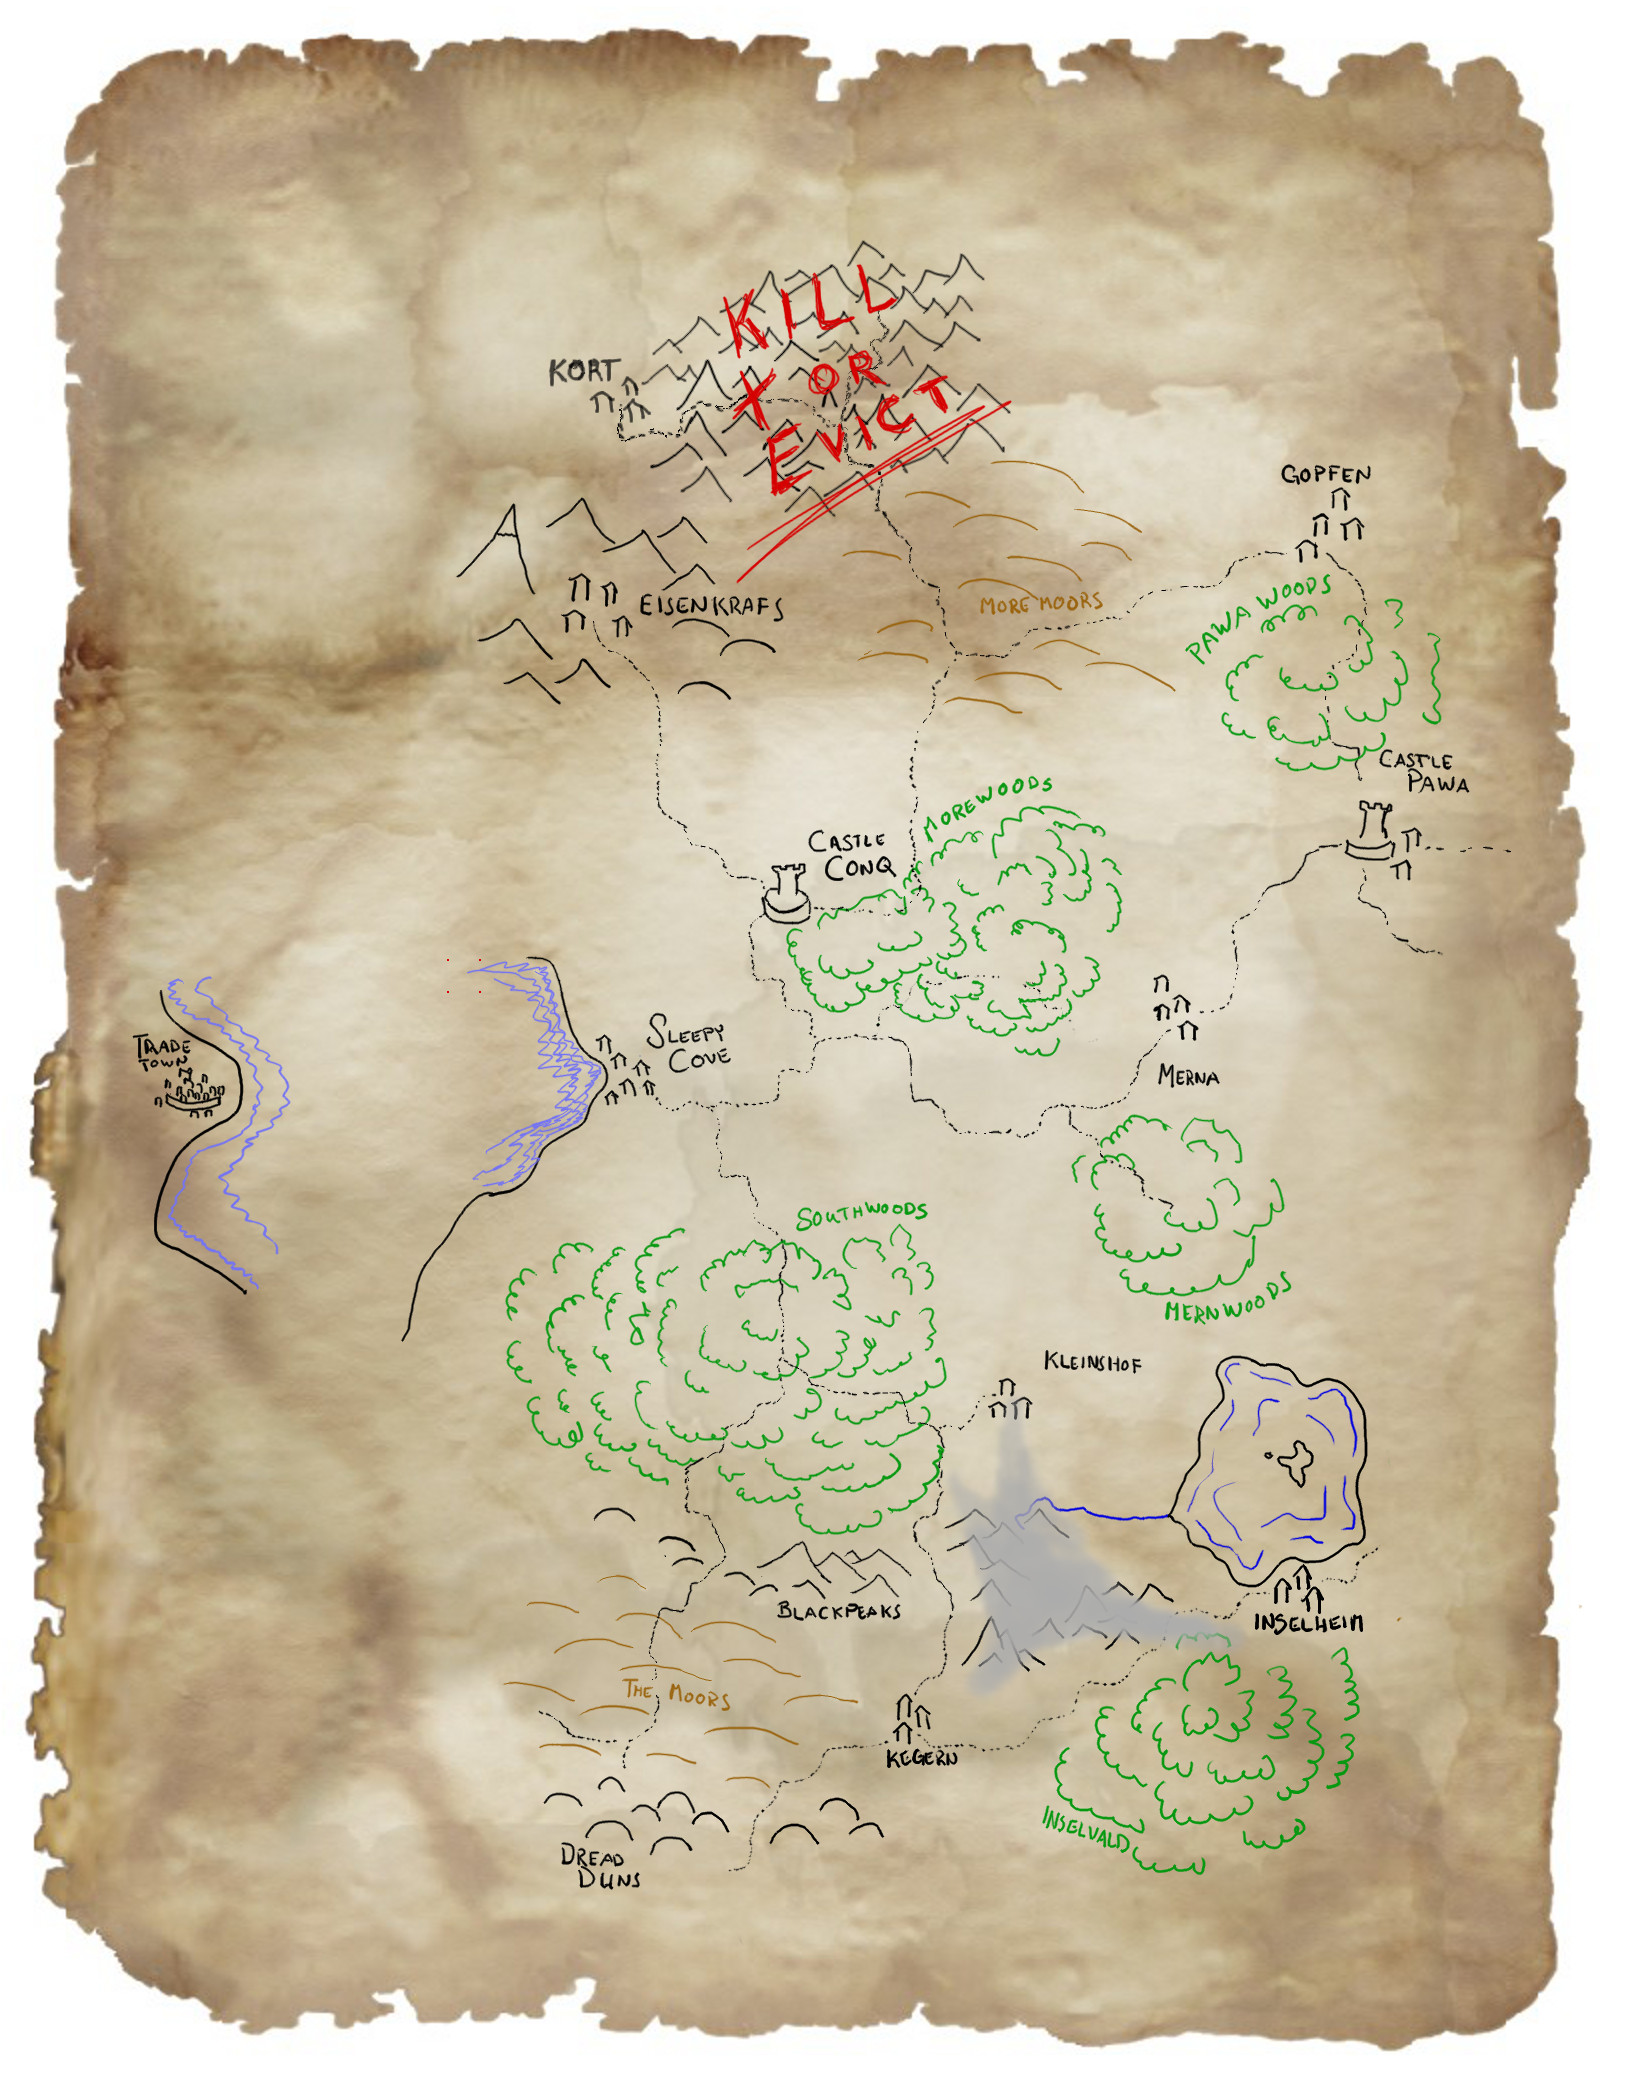
\includegraphics[width=0.999\textwidth]{./map/region-eviction-pl.jpg}
\vfill
\end{samepage}


% GM map
\clearpage                  % right opposing page
\begin{samepage}
\null
\thispagestyle{empty}
\vfill
\noindent
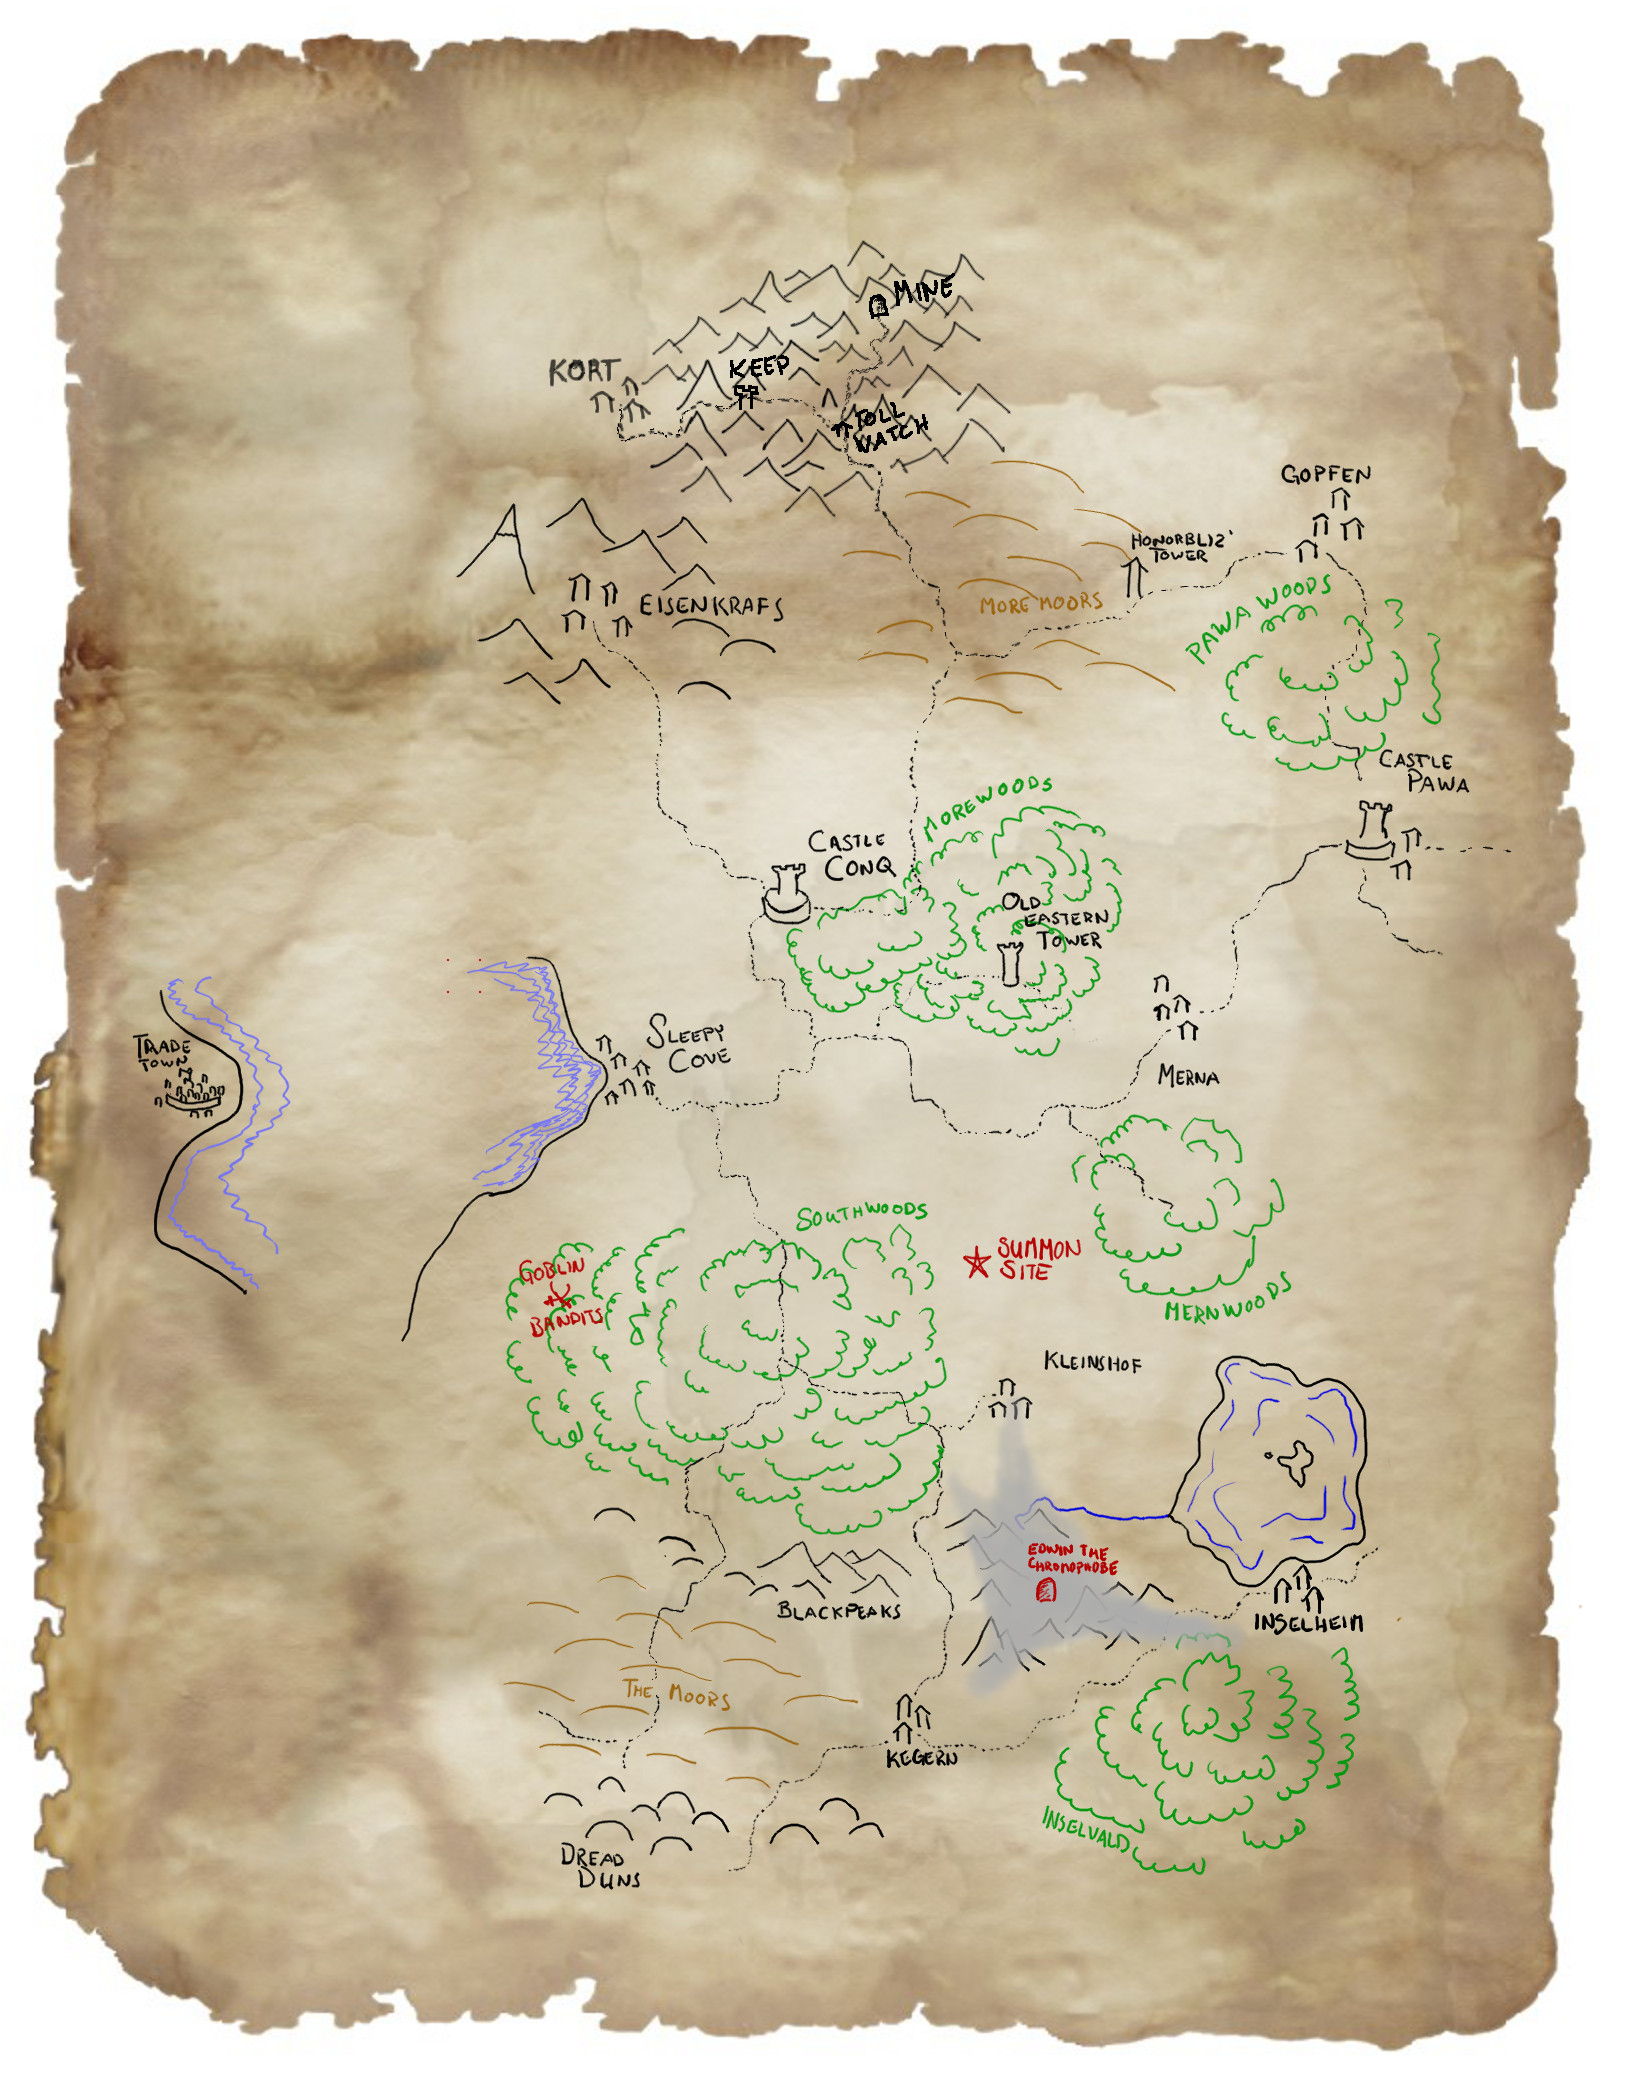
\includegraphics[width=0.999\textwidth]{./map/region-eviction-gm.jpg}
\vfill
\end{samepage}













%--------|---------|---------|---------|---------|---------|---------|---------|
%       10        20        30        40        50        60        70        80
%-------------------------------------------------------------------------------
% fig centered vertically on the rest of final page ?
%----------------------------------------------------
%\vfill
%\noindent
%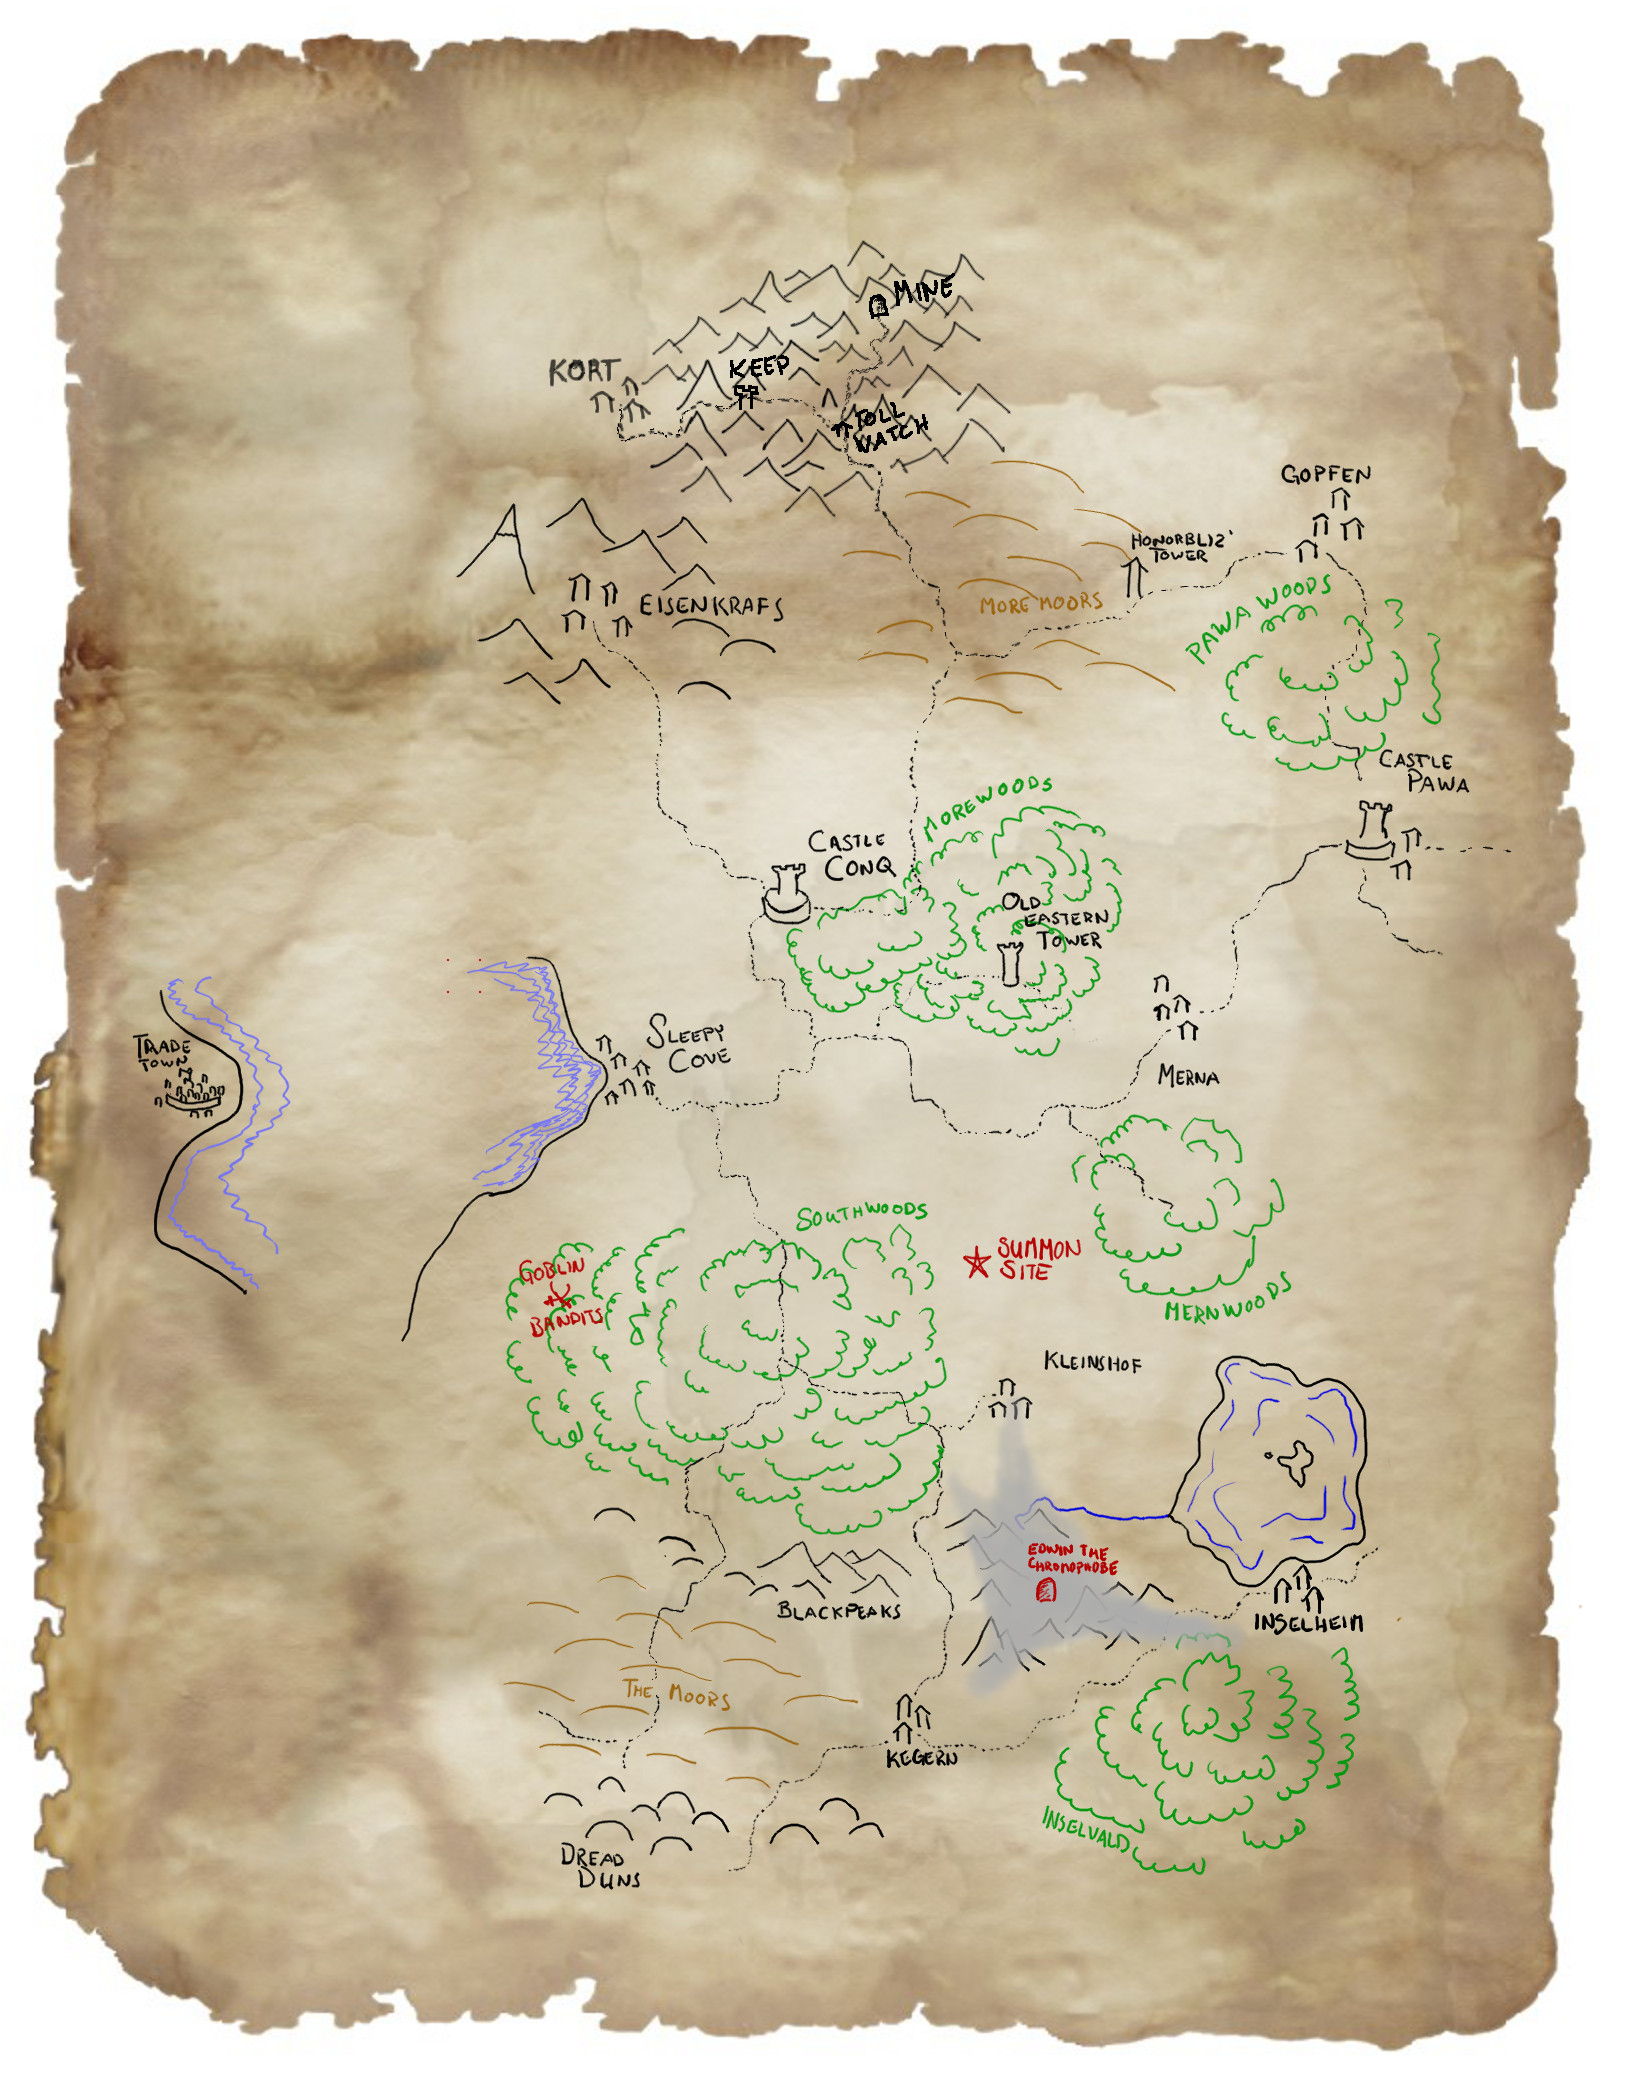
\includegraphics[width=0.999\textwidth]{./map/region-eviction-gm.jpg}
%\vfill






%-------------------------------------------------------------------------------
\end{document}
